%%%%%%%%%%%%%%%%%%%%%%%%%%%%%%%%%%%%%%%%%%%%%%%%%%%%%%%%%%%%%%%%%%%%%%
% amspaper.tex --  LaTeX-based template for submissions to American 
% Meteorological Society journals
%
% Template developed by Amy Hendrickson, 2013, TeXnology Inc., 
% amyh@texnology.com, http://www.texnology.com
% following earlier work by Brian Papa, American Meteorological Society
%
% Email questions to latex@ametsoc.org.
%
%%%%%%%%%%%%%%%%%%%%%%%%%%%%%%%%%%%%%%%%%%%%%%%%%%%%%%%%%%%%%%%%%%%%%
% PREAMBLE
%%%%%%%%%%%%%%%%%%%%%%%%%%%%%%%%%%%%%%%%%%%%%%%%%%%%%%%%%%%%%%%%%%%%%

%% Start with one of the following:
% DOUBLE-SPACED VERSION FOR SUBMISSION TO THE AMS
\documentclass{ametsoc}

% TWO-COLUMN JOURNAL PAGE LAYOUT---FOR AUTHOR USE ONLY
% \documentclass[twocol]{ametsoc}

%%%%%%%%%%%%%%%%%%%%%%%%%%%%%%%%
%%% To be entered only if twocol option is used

\journal{jcli}

\usepackage{color}

%  Please choose a journal abbreviation to use above from the following list:
% 
%   jamc     (Journal of Applied Meteorology and Climatology)
%   jtech     (Journal of Atmospheric and Oceanic Technology)
%   jhm      (Journal of Hydrometeorology)
%   jpo     (Journal of Physical Oceanography)
%   jas      (Journal of Atmospheric Sciences)	
%   jcli      (Journal of Climate)
%   mwr      (Monthly Weather Review)
%   wcas      (Weather, Climate, and Society)
%   waf       (Weather and Forecasting)
%   bams (Bulletin of the American Meteorological Society)
%   ei    (Earth Interactions)

%%%%%%%%%%%%%%%%%%%%%%%%%%%%%%%%
%Citations should be of the form ``author year''  not ``author, year''
\bibpunct{(}{)}{;}{a}{}{,}

%%%%%%%%%%%%%%%%%%%%%%%%%%%%%%%%

%%% To be entered by author:

%% May use \\ to break lines in title:

\title{High-resolution regional climate model evaluation using variable-resolution CESM over California}


%%% Enter authors' names, as you see in this example:
%%% Use \correspondingauthor{} and \thanks{Current Affiliation:...}
%%% immediately following the appropriate author.
%%%
%%% Note that the \correspondingauthor{} command is NECESSARY.
%%% The \thanks{} commands are OPTIONAL.

    \authors{Xingying Huang, \correspondingauthor{Xingying Huang, 
     Department of Land, Air and Water Resources,
     University of California Davis, Davis, CA 95616.}
  Alan M. Rhoades and Paul A. Ullrich}

     \affiliation{Department of Land, Air and Water Resources, University of Califonia, Davis}

\email{xyhuang@ucdavis.edu}


    \extraauthor{Colin M. Zarzycki}
    \extraaffil{National Center for Atmospheric Research}


%%%%%%%%%%%%%%%%%%%%%%%%%%%%%%%%%%%%%%%%%%%%%%%%%%%%%%%%%%%%%%%%%%%%%
% ABSTRACT
%
% Enter your Abstract here

\abstract{Understanding the effect of climate change at regional scales remains a topic of intensive research. Due to computational constraints, the fine horizontal resolutions required to reach regional scales have been largely out of reach for current global climate models. However, high resolution is needed to represent fine-scale processes and topographic forcing, which are a significant driver of local climate variability. Although regional climate models (RCMs) have been widely used at these scales, variable-resolution global climate models (VRGCMs) have arisen as an alternative for studying regional weather and climate. In this paper, the recently developed variable-resolution option within the Community Earth System Model (CESM) is assessed for long-term regional climate modeling. The mean climatology of temperature and precipitation, across California's diverse climate zones, is analyzed and contrasted with the Weather Research and Forcasting (WRF) model (as a traditional RCM), regional reanalysis, gridded observational datasets and a uniform high-resolution CESM with the finite volume (FV) dynamical core. The results show that variable-resolution CESM is competitive in representing regional climatology on both annual and seasonal time scales. This assessment adds value to the use of VRGCMs for projecting climate change over the coming century and improve our understanding of both past and future regional climate related to fine-scale processes. This assessment is also relevant for addressing the scale limitation of current RCMs or VRGCMs when next-generation model resolution increases to $\sim$10km and beyond.} 



\begin{document}


%% Necessary!
\maketitle


%%%%%%%%%%%%%%%%%%%%%%%%%%%%%%%%%%%%%%%%%%%%%%%%%%%%%%%%%%%%%%%%%%%%%
% MAIN BODY OF PAPER
%%%%%%%%%%%%%%%%%%%%%%%%%%%%%%%%%%%%%%%%%%%%%%%%%%%%%%%%%%%%%%%%%%%%%
%
\section{Introduction}

Global climate models (GCMs) have been widely used to simulate both past and future climate. Although GCMs have demonstrated the capability to successfully represent large-scale features of the climate system, they are usually employed at coarse resolutions ($\sim$1$^\circ$), largely due to computational limitations. Global climate reanalysis datasets, which assimilate climate observations using a global model, represent a best estimate of historical weather patterns, but still have relatively coarse resolution no finer than 0.5$^\circ$ (\url{http://reanalyses.org/atmosphere/overview-current-reanalyses}). {\color{red} CFSR is finer than this resolution.} Consequently, regional climate is not well captured by either GCMs or global reanalysis datasets.  However, dynamical processes at unrepresented scales are significant drivers for regional and local climate variability, especially over complex terrain \citep{soares2012wrf}. In order to capture these fine-scale dynamical features, high horizontal resolution is needed to allow for a more accurate representation of fine-scale forcings, processes and interactions \citep{leung2003regional, rauscher2010resolution}. With these enhancements, regional climate data is expected to be more usable for policy makers and local stakeholders in formulating climate adaptation and mitigation strategies.

In order to model regional climate at high spatial and temporal resolution over a limited area, downscaling techniques have been developed. Downscaling techniques can largely be categorized into statistical downscaling and dynamical downscaling. Dynamical downscaling is popular and commonly employed using nested limited-area models (LAMs) or using variable-resolution enabled GCMs (VRGCMs) to model regional scales \citep{laprise2008regional}. In this context, LAMs are typically referred to as regional climate models (RCMs) when used to study climate. Forced by output of GCMs or reanalysis data, RCMs have been widely used, particularly to capture physically consistent regional and local circulations at the needed spatial and temporal scales \citep{leung2003regional, christensen2007regional, bukovsky2009precipitation, mearns2012north}. However, since RCMs only allow one-way coupling with the global domain, there has been growing interest in VRGCMs for modeling regional climate. This approach uses a relatively coarse global model with enhanced resolution over a specific region \citep{staniforth1978variable, fox1997finite}.  Different strategies have been employed for transitioning between coarse and fine resolution regions such as stretched-grid models or grid refinement \citep{fox1997finite, ringler2008multiresolution, skamarock2012multiscale}. VRGCMs have been demonstrated to be effective for regional climate studies and applications at a reduced computational cost compared to uniform GCMs \citep{fox2001variable, fox2006variable, rauscher2013exploring, zarzycki2015effects}. {\color{red}Fox et al. (2000) [Citation]} found that the stretched-grid version of a GCM not only captured large-scale meteorological patterns but also mesoscale features particularly associated with orographic forcing \citep{fox2000uniform}.

%The first is statistical downscaling, which aims to estimate fine scale behavior via analysis of the statistical relationships between observed small-scale variables and larger (GCM) scale variables \citep{fowler2007linking}. This method is empirical and cannot be used if the observed relationships do not hold under a changing climate. Dynamical downscaling, which uses a numerical model to simulate higher spatial resolution conditions in greater detail. 

Compared with RCMs, a key advantage of VRGCMs is that they use a single, unified modeling framework, rather than a separate GCM and RCM. Thus, VRGCMs avoid potential inconsistency between the global and regional domains, and naturally support two-way interaction between these domains without the need for nudging \citep{warner1997tutorial, mcdonald2003transparent, laprise2008challenging, mesinger2013limited}. However, in order to obtain deeper insight into the performance of these two modeling approaches, it is necessary to compare them directly. For the purposes of this paper, we will focus on the recently developed variable-resolution Community Earth System Model (varres-CESM) as our VRGCM of interest. Although CESM has been used heavily for uniform resolution modeling, variable-resolution in the Community Atmosphere Model�s (CAM) Spectral Element (SE) dynamical core has only been recently developed {\color{red}[citation needed]}. \cite{zarzycki2014using} used varres-CESM to show that a high-resolution refinement patch in the Atlantic basin when simulating topical cyclones represented significant improvements over the unrefined simulation. {\color{red}Zarzycki et al. [Citation]} also compared the large-scale features of varres-CESM 0.25$^\circ$ and uniform CESM at 1$^\circ$, and found that adding a refined region over the globe did not noticeably affect the global circulation \citep{zarzycki2014multidecadal, zarzycki2015effects}.

However, varres-CESM has yet to be rigorously investigated for long-term regional climate simulation \citep{taylor2010compatible, zarzycki2014using}.  This paper is the first to investigate whether a VRGCM can show similar or improved ability to model regional climate relative to a traditional RCM {\color{red}This sentence paints the paper as more competitive than it's supposed to be}. The goal of this paper is to evaluate the performance of varres-CESM against gridded observational data, reanalysis data and in comparison to a traditional RCM. In addition, comparisons are drawn with a costly uniform high-resolution CESM simulation \citep{wehner2014resolution}. Our variable-resolution simulations will focus on relatively high resolutions for climate assessment, namely 28km and 14km grid spacing, which are much more typical for dynamically downscaled studies. For comparison with the more widely used RCM method, the Weather Research and Forecasting (WRF) model will be applied at 27km and 9km grid spacing \citep{skamarock2005coauthors}. The study focuses on models' ability to represent current climate statistics, particularly those relative to climate extremes. We anticipate that this assessment will add value in modeling mean regional climatology and improve our understanding about the effects of multi-scale processes in regional climate regulation. Our eventual goal is to utilize these models for assessing future climate and regional climate extremes.

This paper focuses on California (CA) as the study area. With its complex topography, coastal influence, and wide latitudinal range, California is an excellent test bed for regional climate modeling. Further, an understanding of local climate variability is incredibly important for policymakers and stakeholders in California due to its vast agricultural industry, mixed demographics, and vulnerability to anthropogenically-induced climate change \citep{hayhoe2004emissions, cayan2008overview}. RCM simulations over California have also been conducted in previous studies and demonstrated the need for high resolution to better study regional climate and extreme events, especially over complex topography with large climatological gradients \citep{leung2004mid, kanamitsu2007fifty, caldwell2009evaluation, pan2011influences, pierce2013probabilistic}. In particular, \cite{caldwell2009evaluation} presented results from WRF at 12km spatial resolution and showed that although the RCM was effective at simulating the mean climate when compared with observations, some clear biases persisted (such as overestimation of precipitation).

This paper is organized as follows. Section 2 describes the model setup, verification data and evaluation methods. In section 3, simulation results are provided and discussed, with a focus on 2 meter temperature (Ts) and precipitation (Pr). Key results are summarized along with further discussion in section 4.

%In almost all RCM studies, model precipitation was found to be overpredicted over the mountains of the west coast (a point discussed further in Section 3.1). Temperature biases seem to be more model dependent. Based on an intercomparison of 4 different RCM+GCM combinations, Duffy et al. (2006) also investigates model variances and precipitation- temperature correlation. 

%They should present the importance of studying California's climate at the beginning, which would make their objective more understandable. ???

%Among these studies, Kanamitsu et al. (2007) dynamically downscaled reanalysis data to 10-km resolution over CA showing the ability to study various regional climate phenomena within different time scales \citep{kanamitsu2007fifty}.

%paper: Exploring a Multi-resolution Approach Using AMIP Simulations_2015

\section{Models and Methodology}

\subsection{Simulation design} 

All simulations use the AMIP (Atmospheric Model Intercomparison Project) protocols \citep{Gates1992}. AMIP simulations {\color{red}attempt to recreate a climatology similar to that observed over the past few decades [I don't think this is a good characterization]}, with prescribed sea-surface temperatures (SSTs) and sea ice. {\color{red}[More here -- how are SSTs and ice obtained?]}

\subsubsection{Varres-CESM}

CESM is a state-of-the-art Earth modeling framework managed by the National Center for Atmospheric Research (NCAR), consisting of coupled atmospheric, oceanic, land and sea ice models.  CESM has been frequently used for modeling present and future global climate \citep{neale2010description, hurrell2013community}.

The coupling infrastructure in CESM allows the interfacial states and fluxes between the various component models are communicated and the fluxed quantities are conserved. Since we follow AMIP protocols in this study, active communication occurs only between atmospheric and land model. The ocean model and sea ice components are prescribed from data. Here, CAM version 5 (CAM5) \citep{CAM5Tech} and the Community Land Model (CLM) version 4 \citep{CLM40Tech} are used. As mentioned earlier, SE was used as the dynamical core in CAM along with variable-resolution grid support. The FAMIPC5 (F$\_$AMIP$\_$CAM5) compset was chosen for these simulations.

For our study, the variable-resolution cubed-sphere grids are generated for use in CAM and CLM with the open-source software package SQuadGen \citep{ullrich2014squadgen}. The grids used are depicted in Figure \ref{fig:varres-CESM_map}.  The maximum horizontal resolution on these grids are 0.25 degree ($\sim$ 28km) and 0.125 degree ($\sim$ 14km) respectively, with a quasi-uniform 1 degree mesh over the remainder of the globe. Grids are constructed using a paving technique with a 2:1 aspect ratio, so two transition layers are required from 1 degree to 0.25 degree, and one additional transition from 0.25 degree to 0.125 degree. {\color{red} What does this sentence mean? The meteorological patterns (e.g. wind, pressure and precipitation) showed natural and conserved results over the transition boundary as described in \citep{zarzycki2015effects}.} Simulations cover the time period from 1979-01-01 to 2005-12-31 (UTC), although the year 1979 was discarded as the spin-up period. This time period was chosen to provide an adequate sampling of annual variability, to limit computational cost, and for a period where adequate reanalysis data is available for comparison.

Variable-resolution topography files were produced by sampling the National Geophysical Data Center (NGDC) 2-min ($\sim$ 3.5 km) Gridded Global Relief Dataset (ETOPO2v2) topography dataset, followed by application of a differential smoothing technique as described in \cite{zarzycki2015effects}.  Using this technique, the $c$ parameter from Eq. (1) was adjusted to reduce noise in the vertical pressure velocity field. The grid-scale topography is depicted in Figure \ref{fig:topo}. The higher resolution simulations provide a much finer representation of regional topography. This is important for understanding local climate since topography is an important driver for fine-scale dynamic processes, especially over complex terrain.

Land surface datasets, and plant functional types, were created using the $0.5$ degree reference datasets. Greenhouse gas (GHG) concentrations are prescribed based on historical observations. SSTs and ice coverage are supplied by the 1 degree Hadley Centre Sea Ice and Sea Surface Temperature dataset (HadISST) \citep{hurrell2008new}. CAM and CLM tuning parameters are not modified from their default configuration.

%F_AMIP_CAM5 (FAMIPC5)  Description: AMIP run for CMIP5 protocol with cam5 
%How do fields near the refinement boundary look, as compared to uniform resolution? The 2 way interaction of WRF is not conserving, while the 1:2 refinement is conserving. This needs to be discussed and diagnostics near the boundary with respect to conservation done. In particular a comparison of point forecasts and climate averaging needs to be done, to investigate the deviation of the non conserving model and if the climate averaging takes this effect away.

%the time step for different resolutions

\subsubsection{Uniform CESM} 

Output from a globally uniform CESM run at 0.25$^\circ$ spatial resolution is utilized for comparison. It helps us to see if variable-resolution CESM, which is at much lower computation cost than uniform one, can show comparable performance in modeling mean climatology \citep{bacmeister2014exploratory}. This globally uniform simulation uses the CAM5-FV (finite volume) dynamical core and is described in additional detail in \cite{wehner2014resolution} and \cite{wehner2014effect}. {\color{red} need to add details about this and which parameters are different from the public version.} {\color{red}These details should be in one of the wehner2014 papers.  I'm also not sure if uniform CESM should even be included.  Maybe it should be removed.}

%Note that the appendix of the latter paper lists parameters that are different from the public release.

\subsubsection{WRF} 

WRF has been widely used over the past decade for simulating regional climate \citep{lo2008assessment, leung2009atmospheric, soares2012wrf}, and so represents an adequate platform for assessing simulated climatology. In our study, the fully compressible non-hydrostatic WRF model in version 3.5.1 with the Advanced Research WRF (ARW) dynamical solver is used.  WRF is a limited area model that supports nested domains with a typical refinement ratio of 3:1.  The simulation domains of WRF are depicted in Figure \ref{fig:wrf_domains}. Two WRF simulations, representing finest grid resolutions of 27km and 9km, are conducted.  For the WRF 27km simulation, one domain is used. For the WRF 9km simulation, two nested domains are used with the outer domain at 27km (same as the WRF 27km) and inner domain at 9km horizontal grid resolution. Two-way nesting is enabled by overwriting coarse grid data by averaged fine grid data \citep{skamarock2008time}. For both regional simulations,  grids are centered on CA and have 120$\times$110 and 151$\times$172 grid points, respectively. Around the boundaries, 10 grid points are used for lateral relaxation. In order to reduce the drift between forcing data and RCM, grid nudging \citep{stauffer1990use} was applied to the outer domain every 6 hours at all levels except the planetary boundary layer (PBL), as suggested by \cite{lo2008assessment}. This setup uses 41 vertical levels with model top pressure at 50 hPa.

The topography for 27km and 9km simulations are interpolated from USGS (U.S. Geological Survey) elevation data with 10m and 2m {\color{red}Do you mean km?} resolution, respectively. The post-processed grid-scale topography is contrasted in Figure \ref{fig:topo}. Differences between the 28km varres-CESM and 27km WRF model, particularly over the Central Valley, are indicative of a different methodology for preparation of the topography dataset {\color{red}Is there some quantitative assessment of these difference?  L2 difference?}.

Additionally, we used the following physics parameterizations: WSM (WRF Single-Moment) 6-class graupel microphysics scheme \citep{hong2006wrf}, Kain-Fritsch cumulus scheme \citep{kain2004kain}, CAM shortwave and longwave radiation schemes \citep{collins2004description}. These settings are supported by the one-year test running result with different options of cumulus scheme and radiation schemes. For the boundary layer, the Yonsei University scheme (YSU) \citep{hong2006new} and the Noah Land Surface Model \citep{chen2001coupling} were used. Both were chosen as they are common for climate applications that balance long-term reliability and computational cost.

ECMWF Reanalysis (ERA-Interim) data at the surface and on pressure-levels provides initial and lateral conditions for the domains. The lateral conditions and SSTs were updated every 6 hours. ERA-Interim reanalysis ($\sim$80 km) has been widely used and validated for its reliability as forcing data \citep{dee2011era}. Two simulations are conducted with finest horizontal resolution of 27km and 9km respectively, over the same time period as varres-CESM. Again, the year 1979 is used as a spin-up period and is discarded for purposes of analysis. Notably, the $\sim$10 km resolution is actually finer than most previous studies for long-term climate.

%using all the meteorological and static data from nested domains as input.

%\subsection{Topography} 

\subsection{Methodology}

Near surface (2 meter) temperature and precipitation have been analyzed over California to assess the performance of varres-CESM in representing mean climatology. Specifically, our evaluation focuses on daily maximum, minimum and average 2m temperatures (Tmax, Tmin and Tavg) and daily precipitation (Pr). These variables are key for a baseline climate assessment, as a consequence of their close relationship with water resources, agriculture and health. In this context, the biggest impact of weather on California is through heat and precipitation extremes. Since heat extremes dominate during the summer season, we focus on June, July and August (JJA) for assessment of temperature. On the other hand, since the vast majority of precipitation in CA occurs in the winter season (together with the accumulation of snowpack {\color{red}Cite Alan's paper here?}), precipitation over December-January-February (DJF) is emphasized.  Future work will focus on the capability of the variable resolution system to correctly capture the frequency and intensity of heat and precipitation extremes.

%Those seasons also represent the most of the climate variability.

In order to adequately account for natural variability in the mean climate, the simulation period must be chosen appropriately \citep{solomon2007climate}. However, the number of simulated years required for adequate climate statistics depends greatly on the regional climate variability and spatial scale. Past studies have used average weather conditions over a 30-year period to ensure sufficient statistics and avoid imprinting from annual variability \citep{dinse2009climate}. To ensure that our 26-year simulation period is sufficient, {\color{red} we have studied the variability of mean temperature and precipitation in both simulations and observations over 5, 10, 20 and 25 seasons or years, and the results showed that 20 or 25 years' simulation are long enough to adequately capture the regionally climate variability.  \textit{This is the type of vague wording the reviewers will attack us for.  Provide some quantification here.}}

% 30 years or longer run time may sound better, but are not necessary for our case.

The results in the following section are obtained from simulated and observed data over the period 1980-2005.  All datasets have been de-trended so that simulation years can be averaged {\color{red}Did you determine if a trend exists at each grid point?  Or over the whole domain?}  In each case it is found that for temperature a statistically significant trend is present under the two-tailed t-statistic with a significance level of 0.05 {\color{red}What is the magnitude of the trend?  Report these numbers}.  No statistically significant trend was detected for precipitation.

%https://www.ncl.ucar.edu/Document/Functions/Built-in/regCoef-1.shtml
%https://www.ncl.ucar.edu/Document/Functions/Built-in/cdft_p.shtml
%https://www.ncl.ucar.edu/Document/Functions/Built-in/dtrend_msg_n.shtmll; without remove the mean
%However, the linear trend is week with linear regression coefficient averaged around 0.5.

California's rugged topography and large latitudinal extent had led to a diverse variety of climate regions that are poorly captured in typical coarse global climate simulations.  In order to assess the performance of varres-CESM within each region, the state has been divided into five regional zones, including the Central Valley (CV), Mountain Region (MR), North Coast (NC), South Coast (SC), and Desert Region (DR).  The spatial extent of these regions is depicted in Figure \ref{fig:wrf_domains}. The division of these five zones is loosely based on the results of \cite{abatzoglou2009classification} and the climate zones used by the California Energy Commission. To restrict the analysis in each zone, simulations and datasets have been masked to restrict climate variables to each region. 

Standard statistical measures have been used to quantify the performances of the models in comparison with the reference datasets. These statistical variables include the Root-mean-square deviation (RMSD), mean absolute difference (MAD) {\color{red}When you use MAD in the tables, you're using mean difference not mean absolute difference}, mean relative difference (MRD) and correlation, and sample standard deviation. {\color{red}We should include a short description of each of these, such as in the LaTeX comments below.}

%RMSD is defined as the square root of (the sum of the square difference (models-reference) over each grid point of the study area/the numbers of the grid points)
%MAD is defined as the averaged absolute difference (models-reference) over all these grid points
%MRD is defined as the averaged relative difference ((models-reference)/reference) over all these grid points
%correlation is the uncentered pattern correlation, i.e. Pearson product-moment coefficient of linear correlation between models and reference datasets at corresponding locations
%sample standard deviation denoted by $s$, defined as the square root of (the sum of the square difference (x-xbar)/the numbers of the size), here the size are the number of years, the x is the value of each year for each grid point or averaged over each zone.

Grid point differences are calculated by remapping the reference datasets to the model's output grid using bilinear interpolation.  Remapping using patch-based interpolation has also been tested and does not exhibit notable differences.

Student's t-test has been used at the 0.05 significance level to determine if two sets of yearly or seasonally averaged data show statistically significant differences.  Note that this test assumes normality of the sample population {\color{red}It may be necessary to verify approximate normality when this test is applied}.

%T-test 
%http://stattrek.com/regression/slope-test.aspx?Tutorial=AP
%The significance level for a given hypothesis test is a value for which a P-value less than or equal to is considered statistically significant. Typical values for are 0.1, 0.05, and 0.01. These values correspond to the probability of observing such an extreme value by chance.
%t test: https://www.ncl.ucar.edu/Document/Functions/Built-in/ttest.shtml

{\color{red} What about the supplement?}

\subsection{Gridded and Reanalysis Datasets}

For validation purpose, reanalysis and gridded observational datasets of the highest available quality are employed (see Table \ref{tab:Datasets}). In particular, gridded datasets at resolutions finer than 10km  represent the best foundation for assessing the variable-resolution simulation results.  Differences between gridded observations can be due to choice of meteorological stations, interpolation techniques, elevation models and processing algorithms.  Consequently, the use of multiple reference datasets is necessary to understand the uncertainty underlying the observational data.  Moreover, in this study, our purpose of using these products is to serve as realistic proxies to allow for a comparison of the model results. We acknowledge that reanalysis products are particularly sensitive to model choice and choice of assimilated observations and so cannot be treated as truth. Detailed descriptions of these datasets are as follows.

%These data products incorporate station measurements or satellite information and other data. 

\paragraph{NARR:}  The North American Regional Reanalysis (NARR) provides dynamically downscaled data over North America at $\sim$ 32 km resolution and 3 hourly intervals from 1979 through present \citep{mesinger2006north}. It is the National Centers for Environmental Prediction (NCEP)'s high resolution reanalysis product. All major climatological variables are present in NARR, making it an excellent candidate for assessment of regional climate. Nonetheless, some inaccuracies have been identified in NARR that must be accounted for, including deficiencies in precipitation fields away from the continental US \citep{bukovsky2007brief}.

%The NARR model uses the very high resolution NCEP Eta Model (32km/45 layer) together with the Regional Data Assimilation System (RDAS) which, significantly, assimilates precipitation along with other variables. (http://www.esrl.noaa.gov/psd/data/gridded/data.narr.html)

\paragraph{NCEP CPC:} This data set is CPC unified gauge-based analysis of daily precipitation provided by the National Oceanic and Atmospheric Administration (NOAA) Climate Prediction Center (CPC). It is a suite of unified precipitation products with consistent and improved quality by combining all information available at CPC and by taking advantage of the optimal interpolation (OI) objective analysis technique. The gauge analysis covers the Conterminous United States with a fine-resolution at 0.25$^\circ$ from 1948/01/01 to 2006/12/3.

%CPC: National Oceanic and Atmospheric Administration (NOAA) uses more stations than University of Washington (UW); http://www.esrl.noaa.gov/psd/data/gridded/data.unified.daily.conus.html

\paragraph{UW:} The UW daily gridded meteorological data is obtained from the Surface Water Modeling group at the University of Washington \citep{maurer2002long, hamlet2005production}. UW incorporates topographic corrections by forcing the long-term average precipitation to match that of the PRISM dataset. The temperature dataset is produced in a similar fashion as precipitation, but uses a simple 6.1 K/km lapse rate for topographic effect. The dataset is at 0.125$^\circ$ horizontal resolution and is provided from year 1949 to 2010.

\paragraph{PRISM:} The Parameter-elevation Regressions on Independent Slopes Model (PRISM) \citep{daly2008physiographically} supports a 4km gridded dataset obtained by taking a wide range of point measurements and applying a weighted regression scheme that accounts for many factors affecting the local climatology. The datasets include total precipitation and minimum/maximum, (derived) mean temperatures and dewpoints, based on sophisticated quality control measures. Monthly climatological variables are available for 1895 through 2014 provided by the PRISM Climate Group. PRISM is U.S. Department of Agriculture (USDA)'s official climatological data. We will use this product as the main reference dataset for model assessment.

%PRISM is a set of monthly, yearly, and single-event gridded data products of mean temperature and precipitation, max/min temperatures, and dewpoints, primarily for the United States.The PRISM products use a weighted regression scheme to account for complex climate regimes associated with orography, rain shadows, temperature inversions, slope aspect, coastal proximity, and other factors.  PRISM Ts, on the other hand, is based on a larger network of station data and accounts for elevation and topographic effects in a much more sophisticated manner. 

\paragraph{Daymet:}  Daymet is an extremely high resolution (1 km) gridded dataset with daily outputs of total precipitation, humidity, and minimum/maximum temperature covering the years of 1980 through 2013 \citep{thornton1997generating, thornton1999improved, thornton2000simultaneous}. The dataset is produced using an algorithmic technique that ingests point station measurements in conjunction with a truncated Gaussian weighting filter.  Some adjustments are made to account for topography. Daymet is available through the Oak Ridge National Laboratory Distributed Active Archive Center (ORNL DAAC). 

To assess differences in these data products, we have used the Student's t-test to see if the JJA Tmax, Tmin and Tavg from PRISM, UW and Daymet are statistically different from one another {\color{red} Comparing seasonally averaged values, or daily values?}.  For these quantities, all products exhibited similarity at the 0.05 significance level over most regions of the study area, except in the two coastal regions {\color{red}[I'm not sure this means you can assume uncertainty is negligible]}.  A similar assessment was performed for mean DJF precipitation climatology and, in this case, all products exhibited similarity at the 0.05 significance level over the entire simulation domain {\color{red}Even north coast?}.

{\color{red}A figure or table showing these results should be included here.  Can we estimate the uncertainty in these datasets somehow?}

\section{Results}

\subsection{Temperature}

The mean JJA Tmax, Tmin and Tavg climatology over the simulation period, together with NARR and PRISM data is shown in Figure \ref{fig:t2_JJA}.  Statistical measures over CA are tabulated in Table \ref{tab:stat_JJA_t2} {\color{red}How are these calculated?}. All simulations have captured the spatial climate patterns exhibited by the PRISM, with high spatial correlations ($>$0.95), especially for Tmax and Tavg.

For Tmax, when compared with the reference datasets, varres-CESM showed a warm bias of about 2 to 3$^\circ C$. Uniform CESM showed a similar outcome to varres-CESM, but with a larger RMSD value ($\sim$4$^\circ C$). However, WRF produced an overall colder climate, especially the WRF 9km simulation, which were about 2 to 3$^\circ C$ cooler than PRISM. Tmax over CV has been overestimated by all the simulations.  Possible reasons for this overestimation are discussed at the end of this section.

For Tmin, varres-CESM still showed a strong warm bias ($\sim$3 to 4$^\circ C$), with a particularly egregious overestimation over Nevada ($> 5^\circ C$). WRF also exhibited a warm bias, but of a much smaller magnitude ($\sim$2 to 3$^\circ C$). However, the pattern of Tmin presented in Figure \ref{fig:t2_JJA} in both WRF simulations suggests a cooler interior to the Central Valley and warmer perimeter, which is not supported by observations.

For Tavg, the warm bias of Tmin and Tmax by varres-CESM leads a similar overestimation for Tavg. For WRF, underestimation of Tmax and overestimation of Tmin lead to an overall closer match to Tavg over most of the domain, but is indicative of suppressed variability.

The spatial standard deviation of JJA Tmax, Tmin and Tavg by models and PRISM are depicted in Figure \ref{fig:t2_JJA_std}. It can be seen that the variability is largely consistent across different sub-zones, and the values are around 0.5 to 1.5 $^\circ C$ for all the datasets, except for the high Sierras in the WRF 9km simulation which show enhanced variability  ($\sim$2$^\circ C$). {\color{red}It would be interesting to calculate RMSE of the standard deviation.  A visual inspection suggests varres-0.125d has the best representation of variability.}

%the t test of the JJA Tmax, Tmin, Tavg for cesm 0.25d and cesm 0.125d showed they have about half region is significantly the same at the level 0.05.
% (although difference are much smaller when focusing exclusively on California)

Compared with the reference datasets over CA, varres-CESM 0.125 degree produced the lowest RMSD for Tmax, whereas WRF produced the lowest RMSD for Tmin.  In both cases the RMSD was still around 2$^\circ C$.  Notably, Tmin from varres-CESM matched much more closely with NARR, although this may be indicative of a related warm bias in NARR.  In fact, closer examination of the differences between varres-CESM, WRF and NARR marine 2m temperature patterns indicates that CESM and NARR exhibit Tmin values that are approximately $2^\circ C$ larger than WRF.  Since marine 2m temperature is strongly correlated with ocean SSTs, this suggests a possible source of the warm bias in CESM. The sea breeze effect, associated with cooler temperatures near the San Francisco Bay, is apparent in all runs. It is especially encouraging that differences in the varres-CESM simulations, which only used prescribed SSTs, {\color{red}closely match those of WRF}, which were also forced at the lateral domain boundaries with reanalysis data.

%However, these observations are still of the highest quality available and the uncertainty is relatively small compared with difference from the simulations. 
%Varres-CESM overestimated all JJA temperatures (especially Tmin), whereas WRF underestimates Tmax and Tavg.

%The RMSD values between the models and reference datasets range from $\sim$2 to 4$^\circ C$. It can still be seen that varres-CESM is comparable to WRF and uniform CESM, without meaning that they are statistically the same. 

%The DJF climatology is discussed here primarily due to its impact on snowpack. For Tmax (Figure \ref{fig:t2max_DJF}), all simulations show a warm bias over the Central Valley (that is especially pronounced for WRF 27 km), but a cold bias over almost all other regions (particularly in the mountain region of the WRF 9km simulations). For Tmin (Figure \ref{fig:t2min_DJF}), the model simulations show a warm bias over most regions except the mountain region. These errors were evidently smaller when comparing to PRISM rather than UW. For Tavg (lower part of Figure \ref{fig:t2avg_JJA&DJF}), biases are quite smaller between models and PRISM dataset. Overall, the RMSDs are still roughly between 1 and 3 K, as noted in Table \ref{tab:stat_DJF_t2}, but were slightly reduced from summertime RMSDs. Simulations at coarser resolution seem to perform better overall, especially for varres-CESM 0.25$^\circ$ in Tmax, however, varres-CESM 0.25$^\circ$ shows largest error in modeling Tmin. For varres-CESM, biases were largely unaffected by moving to higher resolutions, with a slight underprediction of Tmax and pronounced overprediction of Tmin.  Moving to higher resolutions with WRF greatly increased biases in all cases.

The seasonal cycle of Tavg is shown in Figure \ref{fig:trd_t2avg_allzones} for simulations and reference data from PRISM and NARR {\color{red} How is this calculated?  Do you calculate the standard deviation for each day then average over the month?  Or average the monthly temperatures then calculate the interannual standard deviation?}. Modeled results match closely with reference data with no larger than a 2$^\circ C$ difference, with the largest errors occurring in the summer and winter seasons {\color{red}Statistical significance of differences?}. Compared with PRISM, Varres-CESM overpredicted summer season temperatures in all sub-zones except coastal regions, and underpredicted winter season temperatures in all zones, corresponding to a larger annual temperature range. Uniform CESM was similar to varres-CESM, but with a larger deviation of around 3$^\circ C$. WRF has {\color{red}better performance} in presenting the monthly trend than CESM with about 1$^\circ C$ underestimation over all seasons. There is no clear improvement in the seasonal cycle across resolutions.

Variability in monthly average Tavg is expressed by the sample standard deviation showed in Figure \ref{fig:trd_t2avg_allzones_std}. Generally, standard deviation is between 1 to 2$^\circ C$. Among the simulations, WRF 27km is {\color{red}most consistent with PRISM - How is ``most consistent'' defined?} . WRF 9km is {\color{red}also close to PRISM}, but has $\sim$1$^\circ C$ larger variability over January and February. Varres-CESM basically showed about 0.5$^\circ C$ more scattered values (either above or lower) comparing to reference datasets, and uniform CESM has about 0.5$^\circ C$ lower variability than PRISM.  {\color{red}Are these differences statistically significant?  Use F-test.}

%Due to the disorganized change of monthly variability, it is not easy to interpret this figure.

Due to the impact of summer heat waves, we now focus on Tmax over summer season. In Figure \ref{fig:PDF_t2max_allzones_JJA}, the frequency distribution of Tmax using all JJA daily values over 26 years is depicted. Properties of the frequency distribution, including average, variability, skewness and Kurtosis are tabulated in Table \ref{tab:PDF_t2max_JJA}.  As exemplified by the similarity in the moments of the distribution, varres-CESM clearly captures the general distribution of Tmax correctly.  Outside of the central valley, skewness and Kurtosis measures match closely between varres-CESM and the UW dataset.  In the north and south coastal regions, Daymet overestimates the frequency of cold days leading to deviation in the moments from UW.  Consistent with the observations in Figure \ref{fig:t2_JJA}, outside of the CV WRF tends to be cooler in general and varres-CESM tends to be warmer.  In coastal regions all models show better performance with higher Tmax values than with lower Tmax values; enhanced frequency of cool Tmax values appears to be the primary driver in overestimation of sample variance in these regions.  For both varres-CESM and WRF there is no apparent improvement in statistics at higher resolutions.

In the Central Valley, models show a clear warm bias and underestimated skewness, associated with a long forward tail and temperatures reaching near 50$^\circ C$. As discussed earlier, all models do overestimate Tmax over CV. In order to further assess the accuracy of the gridded observations, we examine the Tmax data directly from recorded weather station observations over the CV. The results validate that Tmax values above 45$^\circ C$ are rare (although station observations suggest these days may be slightly more frequent than suggested by UW and Daymet). The warm bias associated with the aforementioned extreme hot days in both varres-CESM and WRF is likely correlated with overly dry summertime soil moisture, as discussed in \cite{caldwell2009evaluation}. This could be caused by the lack of accurate land surface treatment in climate models. areas. {\color{red}Bonfils and Lobell (2007)} found that irrigation in Central Valley has significantly decreased summertime maximum temperatures especially in heavily-irrigated areas \citep{bonfils2007empirical}. Other studies have also found the cooling effects of irrigation, such as \citep{kueppers2007irrigation}.

%(0.14�C to 0.25�C per decade)

\subsection{Precipitation}

California's Mediterranean climate is associated with heavy precipitation in winter months and drier conditions in summertime.  Agricultural and urban water use in California thus depends on accumulation of wintertime precipitation, which accounts for approximately half of total annual average precipitation.

%50 percent of the $\sim$22.5 inches that California receives for its total annual average precipitation amounts (\url{http://www.ncdc.noaa.gov/cag/}).

The long-term average climatologies of DJF and annual daily precipitation (Pr) over 26 years from simulations and reference datasets are depicted in Figure \ref{fig:pr_DJF_Anuual}. Statistical quantities over CA are given in Table \ref{tab:stat_Pr}. Precipitation is heavily influenced by orography, leading to most accumulation occurring along the North Coast and Sierra Nevada mountains. As with temperature, the model results match the spatial patterns of the PRISM, with high correlation coefficients ($>$0.94).

Along the western edge of the Sierra Nevada and into the CV varres-CESM overestimates total precipitation relative to PRISM, especially in the coarser resolution (28 km) simulation (about 40$\%$-50$\%$) {\color{red}Statistically significant?}.  On the other hand, precipitation is slightly underestimated relative to PRISM along the North Coast, particularly near the Oregon border. {\color{red}Interestingly, varres-CESM 0.125$^\circ$ is statistically the same as PRISM.  [What do you mean?  Be more specific.]} Uniform CESM has {\color{red}slightly better [vague]} results than varres-CESM 0.25deg. There are also notable differences between WRF 27km and WRF 9km. WRF 27km underestimates precipitation along the North Coast (by about 30$\%$) but fairly accurately captures precipitation in the CV, whereas WRF 9km greatly overestimates precipitation (by about 60$\%$-80$\%$) along the North coast and the Sierra Nevada. {\color{red}However, considering the variability shown in the Figure \ref{fig:pr_DJF_Annual_std}, WRF 9km and WRF 27km are both significantly the same at the significance level of 0.05 as PRISM except over the mountain region. [I find this hard to believe -- how did you compute?  if using t-test you should use sample variance from PRISM]}  Notably, variability has a similar pattern to the precipitation intensity, and increases as the precipitation magnitude increases.  The models seem to capture the variation of {\color{red}precipitation well [vague]}, particularly looking at the varres-CESM 0.125deg and WRF 27 km, although variability is $\sim$50$\%$ higher for WRF9km.

Using RMSD values from Table \ref{tab:stat_Pr} as a guide, varres-CESM 0.125$^\circ$ performs slightly better than CESM 0.25$^\circ$ and WRF 27km {\color{red}[Is this all you have to say about the table?]}.

The annual cycle of precipitation averaged over each sub-zone over 26 years is presented in Figure \ref{fig:trd_pr_allzones}. It can be seen that the simulations {\color{red}exhibit similar trends [vague]} to the reference datasets. The main deviation occurred during the rainy seasons, especially in winter. WRF 27km is drier than PRISM and UW, whereas WRF 9km is far wetter in all regions. Varres-CESM {\color{red}tracks well [vague - t-test needed]} with observed precipitation everywhere except in the CV, where precipitation is overestimated at rainy seasons with about 70$\%$-80$\%$. Nonetheless, the strong seasonal dependence on precipitation is apparent with extremely dry conditions during summer months. A slight increase in summertime precipitation is apparent in the Desert region, indicating the North American monsoon. Overall, varres-CESM is {\color{red}more consistent [vague]} with observations compared with WRF. However, we also observe that the peak month for precipitation tends to occur earlier in varres-CESM than in observations {\color{red}[comment on jaggedness of varres-CESM as well]}. {It is not surprising that a seasonal time drift occurred with the varres-CESM simulations as it was not forced by a reanalysis dataset (unlike the WRF simulations). \color{red}[Why?]}

The monthly cycle sample standard deviation is depicted in Figure \ref{fig:trd_pr_allzones_std}. The variability has a similar monthly trend compared to precipitation rate, with overall values from 0 to 4 mm$/$day.  Generally higher inter-annual variability occurs over locations of higher mean precipitation \ref{fig:trd_pr_allzones}. Comparing with observations, varres-CESM exhibited a {\color{red}slightly larger variability [vague]} (basically no more than 1mm$/$day) in the rainy season, while WRF 27km has better representation with {\color{red}a little lower values [vague]}. WRF 9km again showed larger variability (about $\sim$1mm$/$day more) during rainy seasons over most regions. Such higher variability within higher magnitude of precipitation has also been found in previous studies; for example,\cite{duffy2006simulations} observe higher variability associated with higher spatial resolution in RCMs, attributed to a more accurate representation of topography. The main cause of the interannual variability of precipitation over CA is the El Ni\~{n}o�Southern Oscillation (ENSO), which varies the amount of moisture flux transported to this region. {\color{red}[Show statistical significance of differences in variability via f-test]}

%The primary source of interannual variability in the study region is El Ni�o�Southern Oscillation (ENSO), which introduces variability primarily on times scales of 4 to 7 yr. This affects spatially averaged precipitation in the study region by varying the amount of moisture advected into the region.

The frequency distribution of DJF Pr has been constructed from rainy days in winter (Pr$>$=0.1mm/d) and depicted in Figure \ref{fig:PDF_pr_allzones_DJF}. Generally, varres-CESM matches more closely with observations everywhere except in the CV {\color{red}[give p-value of  a two-sample Kolmogorov-Smirnoff test]}. In this region WRF 27km appears to better capture high-intensity precipitation events, but performs poorly on low-intensity events (Pr$<$20 mm/d). The underestimation of rainfall frequency in WRF 27km appears consistent across regions. WRF 9km produces a significantly better treatment of low-intensity events, but greatly overestimates the frequency of high-intensity events (Pr$>$20 mm/d). Notably, varres-CESM 0.25 degree and varres-CESM 0.125 degree are not significantly different {\color{red}[give p-value of a two-sample K-S test]}. For strong precipitation events, varres-CESM and WRF 27km show {\color{red}good performance [vague]} over most regions except in those noted above, although these conclusions are also constrained by observational uncertainty {\color{red}[Should we even mention this given we can't quantify it?]}.

The overestimation of precipitation for WRF at high resolution has also been found in previous studies. Although not as pronounced, \cite{caldwell2009evaluation} demonstrated that WRF at 12km largely overestimated the precipitation over the California's mountainous regions (however, this paper did employ a different set of parameterizations).  The exact cause of this overprediction has yet to be identified in the literature and a comprehensive analysis of the cause of these errors is beyond the scope of this paper. Further discussion can be found in former studies that employ different microphysics schemes (and so produce a wide range of precipitation magnitudes) including \citep{leung2003hydroclimate, jankov2005impact, gallus2006comparison, chin2010preliminary, caldwell2010california}.

A concise summary of model performance over CA is provided by the Taylor diagram (Figure \ref{fig:taylor_diagram}). This diagram includes the spatially centered correlation between the simulated and observed fields, the RMS variability of simulations normalized by that in the observations, and mean differences from reference data. It can be seen that the models correlate well with the PRISM reference dataset. Normalized standard deviation and bias are larger for precipitation, especially for WRF 9km. Overall, varres-CESM has demonstrated that it can competitively compare to WRF in capturing the regional climatology of California. ({\color{red}update the plot})

\section{Discussions and summary}

The need for high resolution model data to address regional climate change and extreme events has motivated the development of new modeling tools.  Our study investigated the use of a variable-resolution GCM (i.e. varres-CESM) as an alternative approach for two-way dynamically downscaled climate modeling. The performance of varres-CESM was evaluated in simulating California's unique regional climatology. This relatively new technique has been evaluated against gridded reference datasets, regional reanalysis data and the Weather Research and Forecasting model.

%To achieve this goal, uniform CESM is also included together with gridded reference datasets

Based on 26 years of high-resolution historical climate simulations, we analyzed the mean climatology of California and across its climate divisions from both temperature and precipitation. Generally, when compared with gridded observational datasets, both varres-CESM and WRF do a good job of capturing regional climatological patterns with high spatial correlations ($>$0.94). Uncertainty between reference datasets exists, but is relatively small and not statistically significant over most regions. We found that varres-CESM showed comparable performance as WRF in regional climate study. Even compared with a uniform high-resolution GCM (CESM-FV), varres-CESM also performed competitively.
%In the meantime, a uniform CESM simulation is also included. High-quality gridded datasets are used as reference datasets. 

Deviations from reference datasets do exist in these simulations, but they have different features. During summer, varres-CESM model possessed about 2 to 3$^\circ C$ warmer climate, especially in the Central Valley. WRF exhibited a colder ($\sim$2$^\circ C$) Tmax over most regions except the Central Valley, but a little warmer in Tmin. Overall, varres-CESM showed better ability in reproducing mean climatology of Tmax, but WRF was better at modeling Tmin and Tavg. The variability of JJA mean temperature is largely within the range of 0.5 to 1.5$^\circ C$. WRF presents the annual cycle of Tavg better than CESM with about 1$^\circ C$ underestimation. CESMs showed about 2$^\circ C$ overestimation of Tavg over the summer season and similar magnitude of underestimation over winter season, indicating larger temperature range over most regions.

When assessing the representation of temperature, both varres-CESM and WRF 27km exhibit {\color{red}close frequency [?]} to observations over all study area except in Central Valley (CV). The failure to correctly capture CV Tmax is likely caused by the lack of irrigation cooling effect over this region. Future work will address this issue by adding an irrigation parameterization to varres-CESM so as to figure out the role irrigation played in regulating Tmax, and the overestimation and longer upbounded tail of frequency distribution for Tmax,

As for precipitation representation, varres-CESM matches closely with PRISM everywhere except for an overestimation of winter or annual precipitation (about 40$\%$-50$\%$) along the western side of Sierra Nevada and into the CV.  Increasing the resolution produces a slight reduction in this overestimation (10$\%$) likely due to improved treatment of orographic effects. WRF 27km underestimates precipitation (about 30$\%$) along the North coast and Sierra Nevada mountains, where almost all the precipitation comes from, whereas WRF 9km shows a large overestimation (about 70$\%$$-$80$\%$). Variability of precipitation ranges from 0 to 6 mm$/$day, with generally higher inter-annual variability over locations of higher mean precipitation. For strong precipitation events probalibity, varres-CESM and WRF 27km show {\color{red}satisfactory [vague]} modeling ability over most regions (except at the CV for varres-CESM), {\color{red}although the reference datasets also show some uncertainties [see earlier comment]}.

%with main deviation occurred during the rainy seasons. Varres-CESM also exhibited a slightly larger variability than WRF 27km.  
%The main precipitation modeling deviations occurred during rainy seasons, especially in winter. 

Higher resolution (0.125$^\circ$) simulation of varres-CESM do show better results in capturing summer Tmax, precipitation and their variablility, than the coarser resolution run. However, the improvements are not statistically significant. For WRF, when resolution increased, the model produces obviously overestimated precipitation as previous studies have also found when using RCMs for fine-scale simulations as aforementioned. The use convection scheme is perhaps not needed when grid spacing is near 10km. However, it turned out that almost all of the precipitation comes from resolved (large-scale) processes for all these models. In this way, model deviation is mainly related with resolved-scale processes and microphysics scheme plays a major role, which makes it necessary to develop more scale-aware parameterizations. 

%Since our grid spacing is approaching the 10 km bound beyond which subgrid-scale (commonly referred to as �convective�) parameterizations are perhaps not needed (e.g. Dudhia et al. 2003).

The importance and necessity of high resolution for regional climate studies has been widely stressed by previous studies. However, whether the current regional climate models can fulfill this demand when resolution is pushed to local scales is questionable. It is clear that further work is urgently needed to solve the scale limitation of current regional climate models at fine horizontal resolutions. The possible causes of the scale limitation may include a lack of accurate scare-aware physical parameterizations near or below 10 km horizontal resolution, the treatment of dynamics at fine scales, and the interactions among different components of RCMs or VRGCMs (e.g., land-atmosphere interactions). 

%A model�s performance can depend on horizontal resolution for different reasons: a more accurate representation of fine scale forcings (e.g. topography and land use), the better representation of processes and interactions (e.g. the dynamical structure of weather systems or cloud complexes; the location of major circulation features), and the direct dependence of physical parameterizations on the model grid size and time step interval.

In summary, varres-CESM demonstrated competitive utility for studying high-resolution regional climatology when compared to a regional climate model (WRF) and a uniform high-resolution GCM (CESM-FV). Deviations, showed within these models, are not indicative of deep underlying problems with the model formulation, but one should be aware of these differences when using these models for assessing future climate change. This study suggests that variable-resolution GCMs are useful tools for assessing climate change over the coming century. As the need for assessments of regional climate change is increasing, alternative modeling strategies, including variable-resolution global climate models will be needed to improve our understanding of the effects of fine-scale processes representation in regional climate regulation.


%%%%%%%%%%%%%%%%%%%%%%%%%%%%%%%%%%%%%%%%%%%%%%%%%%%%%%%%%%%%%%%%%%%%%
% ACKNOWLEDGMENTS
%%%%%%%%%%%%%%%%%%%%%%%%%%%%%%%%%%%%%%%%%%%%%%%%%%%%%%%%%%%%%%%%%%%%%
\acknowledgments

The authors would like to thank Michael Wehner and Da\'ith\'i Stone for providing the uniform resolution CESM dataset. We would further like to thank Travis O'Brien for his many useful conversations on climate model assessment. We also want to thank Xuemeng Chen for her assistance in WRF running. This project is supported in part by the University of California, Davis and by the Department of Energy ``Multiscale Methods for Accurate, Efficient, and Scale-Aware Models of the Earth System'' program.

 \bibliographystyle{ametsoc2014}
 \bibliography{database2015}

%\section{Figures and tables}

% TABLES

%%%%%%%%%%%Table1%%%%%%%%%%%%%%%%%%%%%%%
\begin{table}
\caption{Reanalysis and statistically downscaled observational datasets used in this study.} \label{tab:Datasets}
\begin{center}
\begin{tabular}{lcccc}
\hline \textbf{Data source} & \textbf{Variables used} & \textbf{Spatial resolution} & \textbf{Temporal resolution} \\
\hline \textbf{NARR} & Pr, T$_{s}$ & 32km & daily, 3-hourly \\
\textbf{NCEP CPC} & Pr & 0.25$^\circ$ & daily \\
\textbf{UW} & Pr, T$_{min}$, T$_{max}$ & 0.125$^\circ$ & daily \\
\textbf{PRISM} & Pr, T$_{min}$, T$_{max}$, T$_{avg}$ & 4km & monthly \\
\textbf{Daymet} & Pr, T$_{min}$, T$_{max}$ & 1km & daily \\
\hline
\end{tabular}
\end{center}
\end{table}


%%%%%%%%%%%Table2%%%%%%%%%%%%%%%%%%%%%%%
\begin{table}
\begin{center}
\caption{RMSD, MAD and Correlation (Corr) for {\color{red}seasonally-averaged} JJA temperature metrics over California} \label{tab:stat_JJA_t2}
\begin{tabular}{lcccc}
\hline \textbf{RMSD} & \textbf{UW}  & \textbf{PRISM} & \textbf{Daymet} \\
\hline $    $ & T$_{max}$ $\     $  T$_{min}$ & T$_{max}$ $\     $  T$_{min}$ $\     $ T$_{avg}$& T$_{max}$ $\     $  T$_{min}$\\
\hline \textbf{varres-CESM 0.25d} & 2.322 $\ $ 3.745 & 2.924 $\ $ 3.121 $\ $ 2.604 & 2.810 $\ $ 3.934 \\
\textbf{varres-CESM 0.125d} & 1.900 $\ $ 3.631 & 2.447 $\ $ 2.944 $\ $ 2.184 & 2.475 $\ $ 3.701 \\
\textbf{WRF 27km} & 2.310 $\ $ 2.738 & 2.933 $\ $ 2.254 $\ $ 2.169 & 2.511 $\ $ 2.992 \\
\textbf{WRF 9km} & 3.319 $\ $ 2.937 & 3.492 $\ $ 1.837 $\ $ 1.769 & 3.203 $\ $ 2.942 \\
\textbf{uniform CESM 0.25d} & 3.885 $\ $ 4.088 & 4.265 $\ $ 3.614 $\ $ 3.536 & 4.315 $\ $ 4.274 \\
\hline
\end{tabular}

\begin{tabular}{lcccc}
\hline \textbf{MAD} & \textbf{UW}  & \textbf{PRISM} & \textbf{Daymet} \\
\hline $    $ & T$_{max}$ $\     $  T$_{min}$ & T$_{max}$ $\     $  T$_{min}$ $\     $ T$_{avg}$& T$_{max}$ $\     $  T$_{min}$\\
\hline \textbf{varres-CESM 0.25d} & 0.981 $\ $ 2.907 & 0.606 $\ $ 1.731 $\ $ 0.823 & 1.177 $\ $ 2.877 \\
\textbf{varres-CESM 0.125d} & 0.645 $\ $ 2.848 & 0.203 $\ $ 1.660 $\ $ 0.579 & 0.818 $\ $ 2.744 \\
\textbf{WRF 27km} & -0.577 $\ $ 0.819 & -0.952 $\ $ -0.357 $\ $ -0.771 & -0.386 $\ $ 0.789 \\
\textbf{WRF 9km} & -2.277 $\ $ 1.862 & -2.720 $\ $ 0.674 $\ $ -1.142 & -2.103 $\ $ 1.757 \\
\textbf{uniform CESM 0.25d} & 1.812 $\ $ 2.993 & 1.449 $\ $ 1.815 $\ $ 1.280 & 2.013 $\ $ 2.961 \\
\hline
\end{tabular}

\begin{tabular}{lcccc}
\hline \textbf{Corr} & \textbf{UW}  & \textbf{PRISM} & \textbf{Daymet} \\
\hline $    $ & T$_{max}$ $\     $  T$_{min}$ & T$_{max}$ $\     $  T$_{min}$ $\     $ T$_{avg}$& T$_{max}$ $\     $  T$_{min}$\\
\hline \textbf{varres-CESM 0.25d} & 0.998 $\ $ 0.982 & 0.996 $\ $ 0.986 $\ $ 0.994 & 0.997 $\ $ 0.979 \\
\textbf{varres-CESM 0.125d} & 0.998 $\ $ 0.985 & 0.997 $\ $ 0.988 $\ $ 0.996 & 0.997 $\ $ 0.983 \\
\textbf{WRF 27km} & 0.997 $\ $ 0.982 & 0.996 $\ $ 0.989 $\ $ 0.996 & 0.997 $\ $ 0.978 \\
\textbf{WRF 9km} & 0.996 $\ $ 0.985 & 0.997 $\ $ 0.993 $\ $ 0.998 & 0.996 $\ $ 0.984 \\
\textbf{uniform CESM 0.25d} & 0.994 $\ $ 0.980 & 0.992 $\ $ 0.981 $\ $ 0.991 & 0.993 $\ $ 0.977 \\
\hline
\end{tabular}
\end{center}
\end{table}

%%%%%%%Table3%%%%%%%%%%%%%%%%%%%%%%%%%%%%%%

\begin{table}
\begin{center}
\caption{The first four moments of the JJA Tmax frequency in each sub-zone.  Column titles refer to Average (Avg), Variance (Var), Skewness (Skew) and Kurtosis (Kurt).} \label{tab:PDF_t2max_JJA}
\begin{tabular}{lccccc}
\hline \textbf{} & \textbf{Central valley}  & \textbf{Mountain} & \textbf{North coast} & \textbf{South coast} &\textbf{Desert}\\
\hline & Avg $\ $\ $ Var$\ $\ $Skew$\ $\ $ Kurt$ & Avg $\ $\ $ Var$\ $\ $Skew$\ $\ $ Kurt$  & Avg $\ $\ $ Var$\ $\ $Skew$\ $\ $ Kurt$  & Avg $\ $\ $ Var$\ $\ $Skew$\ $\ $ Kurt$  & Avg $\ $\ $ Var$\ $\ $Skew$\ $\ $ Kurt$  \\
\hline \textbf{UW} &32.6$\ $	24.8	$\ $-0.8$\ $	0.9	&	26.7	$\ $33.2$\ $	-0.4	$\ $0.3	&	25.9	$\ $30.4	$\ $0.1$\ $	-0.5		&25.9$\ $	30.4	$\ $0.1$\ $	-0.5&		37.0	$\ $22.9$\ $	-0.6	$\ $0.7\\
\textbf{Daymet} & 32.7$\ $	23.5$\ $	-0.9$\ $	1.5	&	25.9	$\ $39.3$\ $	-0.5$\ $	0.5	&	26.5	$\ $30.1	$\ $-0.3$\ $	0.4	&	26.5	$\ $30.1	$\ $-0.3	$\ $0.4		& 37.0	$\ $24.3	$\ $-0.6$\ $	0.6\\
\hline\textbf{CESM 0.25d}& 34.1$\ $	26.2	$\ $-0.4$\ $	0.2	&	28.1	$\ $27.6$\ $	-0.4$\ $	0.3	&	26.4	$\ $37.4	$\ $0.1$\ $	-0.7		& 26.4$\ $	37.4	$\ $0.1$\ $	-0.7	&	37.6$\ $	19.0$\ $	-0.5	$\ $0.8\\
\textbf{CESM 0.125d}& 34.3	$\ $28.5$\ $	-0.5	$\ $0.4	&	27.2	$\ $30.0$\ $	-0.4$\ $	0.3	&	26.3	$\ $37.4$\ $	0.1$\ $	-0.6		& 26.3$\ $	37.4$\ $	0.1	$\ $-0.6		& 37.3	$\ $21.3$\ $	-0.5	$\ $0.4\\
\hline\textbf{WRF 27km} & 33.9	$\ $34.8	$\ $-0.5$\ $	0.2	&	24.9	$\ $34.8$\ $	-0.3	$\ $0.0	&	26.0	$\ $36.7	$\ $-0.1$\ $	-0.5		& 26.0$\ $	36.7	$\ $-0.1	$\ $-0.5		& 36.5$\ $	22.6$\ $	-0.6$\ $	0.5\\
\textbf{WRF 9km}&32.4		$\ $33.1	$\ $	-0.7	$\ $	0.6	&	22.4		$\ $38.5		$\ $-0.5		$\ $0.6	&	24.9	$\ $	32.6		$\ $0.0		$\ $-0.6	&	24.9	$\ $	32.6	$\ $	0.0		$\ $-0.6	&	34.4		$\ $24.4		$\ $-0.5		$\ $0.4\\
\hline
\end{tabular}
\end{center}
\begin{tabular}{p{6in}}
\textbf{Notes:} If skew $>0$ [skew $<0$], the distribution trails off to the right [left]. If kurtosis $> 0$ [$<0$], it is usually more sharply peaked [flatter] than the normal distribution (leptokurtic and platykurtic, respectively).
\end{tabular}
\end{table}

%%%%%%Table4%%%%%%%%%%%%%%%%%%%%%%%%%%%

\begin{table}
\begin{center}
\caption{RMSD, MAD, MRD, Correlation (Corr) for precipitation over California} \label{tab:stat_Pr}
\begin{tabular}{lcccc}
\hline \textbf{Annual} & \textbf{CPC}  & \textbf{UW} & \textbf{PRISM} & \textbf{DAYMET} \\
\hline $    $ & RMSD $\ $ MAD $\ $ MRD $\ $ Corr & RMSD $\ $ MAD $\ $ MRD $\ $ Corr & RMSD $\ $ MAD $\ $ MRD $\ $ Corr & RMSD $\ $ MAD $\ $ MRD $\ $ Corr \\
\hline \textbf{varres-CESM 0.25d} & 0.607 $\ $ 0.394 $\ $ 0.413 $\ $ 0.981 & 0.616 $\ $ 0.292 $\ $ 0.434 $\ $ 0.968 & 0.727 $\ $ 0.203 $\ $ 0.429 $\ $ 0.952 & 0.567 $\ $ 0.191 $\ $ 0.375 $\ $ 0.972 \\
\textbf{varres-CESM 0.125d} & 0.469 $\ $ 0.207 $\ $ 0.321 $\ $ 0.980 & 0.526 $\ $ 0.115 $\ $ 0.339 $\ $ 0.970 & 0.624 $\ $ 0.045 $\ $ 0.328 $\ $ 0.961 & 0.504 $\ $ 0.027 $\ $ 0.310 $\ $ 0.973 \\
\textbf{WRF 27km} & 0.419 $\ $ -0.205 $\ $ 0.269 $\ $ 0.977 & 0.580 $\ $ -0.308 $\ $ 0.274 $\ $ 0.971 & 0.765 $\ $ -0.396 $\ $ 0.296 $\ $ 0.965 & 0.647 $\ $ -0.409 $\ $ 0.312 $\ $ 0.970 \\
\textbf{WRF 9km} & 2.226 $\ $ 1.485 $\ $ 0.950 $\ $ 0.957 & 2.052 $\ $ 1.393 $\ $ 0.864 $\ $ 0.964 & 1.889 $\ $ 1.322 $\ $ 0.815 $\ $ 0.970 & 2.005 $\ $ 1.306 $\ $ 0.773 $\ $ 0.961 \\
\textbf{uniform CESM 0.25d} & 0.555 $\ $ 0.134 $\ $ 0.277 $\ $ 0.969 & 0.600 $\ $ 0.031 $\ $ 0.302 $\ $ 0.961 & 0.700 $\ $ -0.057 $\ $ 0.290 $\ $ 0.953 & 0.600 $\ $ -0.069 $\ $ 0.284 $\ $ 0.962 \\
\hline
\end{tabular}

\begin{tabular}{lcccc}
\hline \textbf{DJF} & \textbf{CPC}  & \textbf{UW} & \textbf{PRISM} & \textbf{DAYMET} \\
\hline $    $ & RMSD $\ $ MAD $\ $ MRD $\ $ Corr & RMSD $\ $ MAD $\ $ MRD $\ $ Corr & RMSD $\ $ MAD $\ $ MRD $\ $ Corr & RMSD $\ $ MAD $\ $ MRD $\ $ Corr \\
\hline \textbf{varres-CESM 0.25d} & 1.486 $\ $ 0.986 $\ $ 0.532 $\ $ 0.972 & 1.445 $\ $ 0.673 $\ $ 0.531 $\ $ 0.959 & 1.654 $\ $ 0.577 $\ $ 0.547 $\ $ 0.943 & 1.346 $\ $ 0.514 $\ $ 0.435 $\ $ 0.964 \\
\textbf{varres-CESM 0.125d} & 1.194 $\ $ 0.638 $\ $ 0.396 $\ $ 0.976 & 1.234 $\ $ 0.346 $\ $ 0.398 $\ $ 0.965 & 1.395 $\ $ 0.287 $\ $ 0.400 $\ $ 0.955 & 1.170 $\ $ 0.212 $\ $ 0.337 $\ $ 0.969 \\
\textbf{WRF 27km} & 0.888 $\ $ -0.376 $\ $ 0.269 $\ $ 0.975 & 1.289 $\ $ -0.688 $\ $ 0.289 $\ $ 0.967 & 1.552 $\ $ -0.785 $\ $ 0.298 $\ $ 0.962 & 1.351 $\ $ -0.848 $\ $ 0.324 $\ $ 0.966 \\
\textbf{WRF 9km} & 4.264 $\ $ 2.607 $\ $ 0.742 $\ $ 0.950 & 3.835 $\ $ 2.315 $\ $ 0.616 $\ $ 0.955 & 3.570 $\ $ 2.256 $\ $ 0.604 $\ $ 0.964 & 3.804 $\ $ 2.183 $\ $ 0.554 $\ $ 0.955 \\
\textbf{uniform CESM 0.25d} & 1.392 $\ $ 0.377 $\ $ 0.300 $\ $ 0.960 & 1.431 $\ $ 0.064 $\ $ 0.316 $\ $ 0.951 & 1.544 $\ $ -0.033 $\ $ 0.314 $\ $ 0.946 & 1.406 $\ $ -0.095 $\ $ 0.288 $\ $ 0.953 \\
\hline
\end{tabular}
\end{center}
\end{table}

%\subsection{Figures}

\begin{figure}
\begin{center}
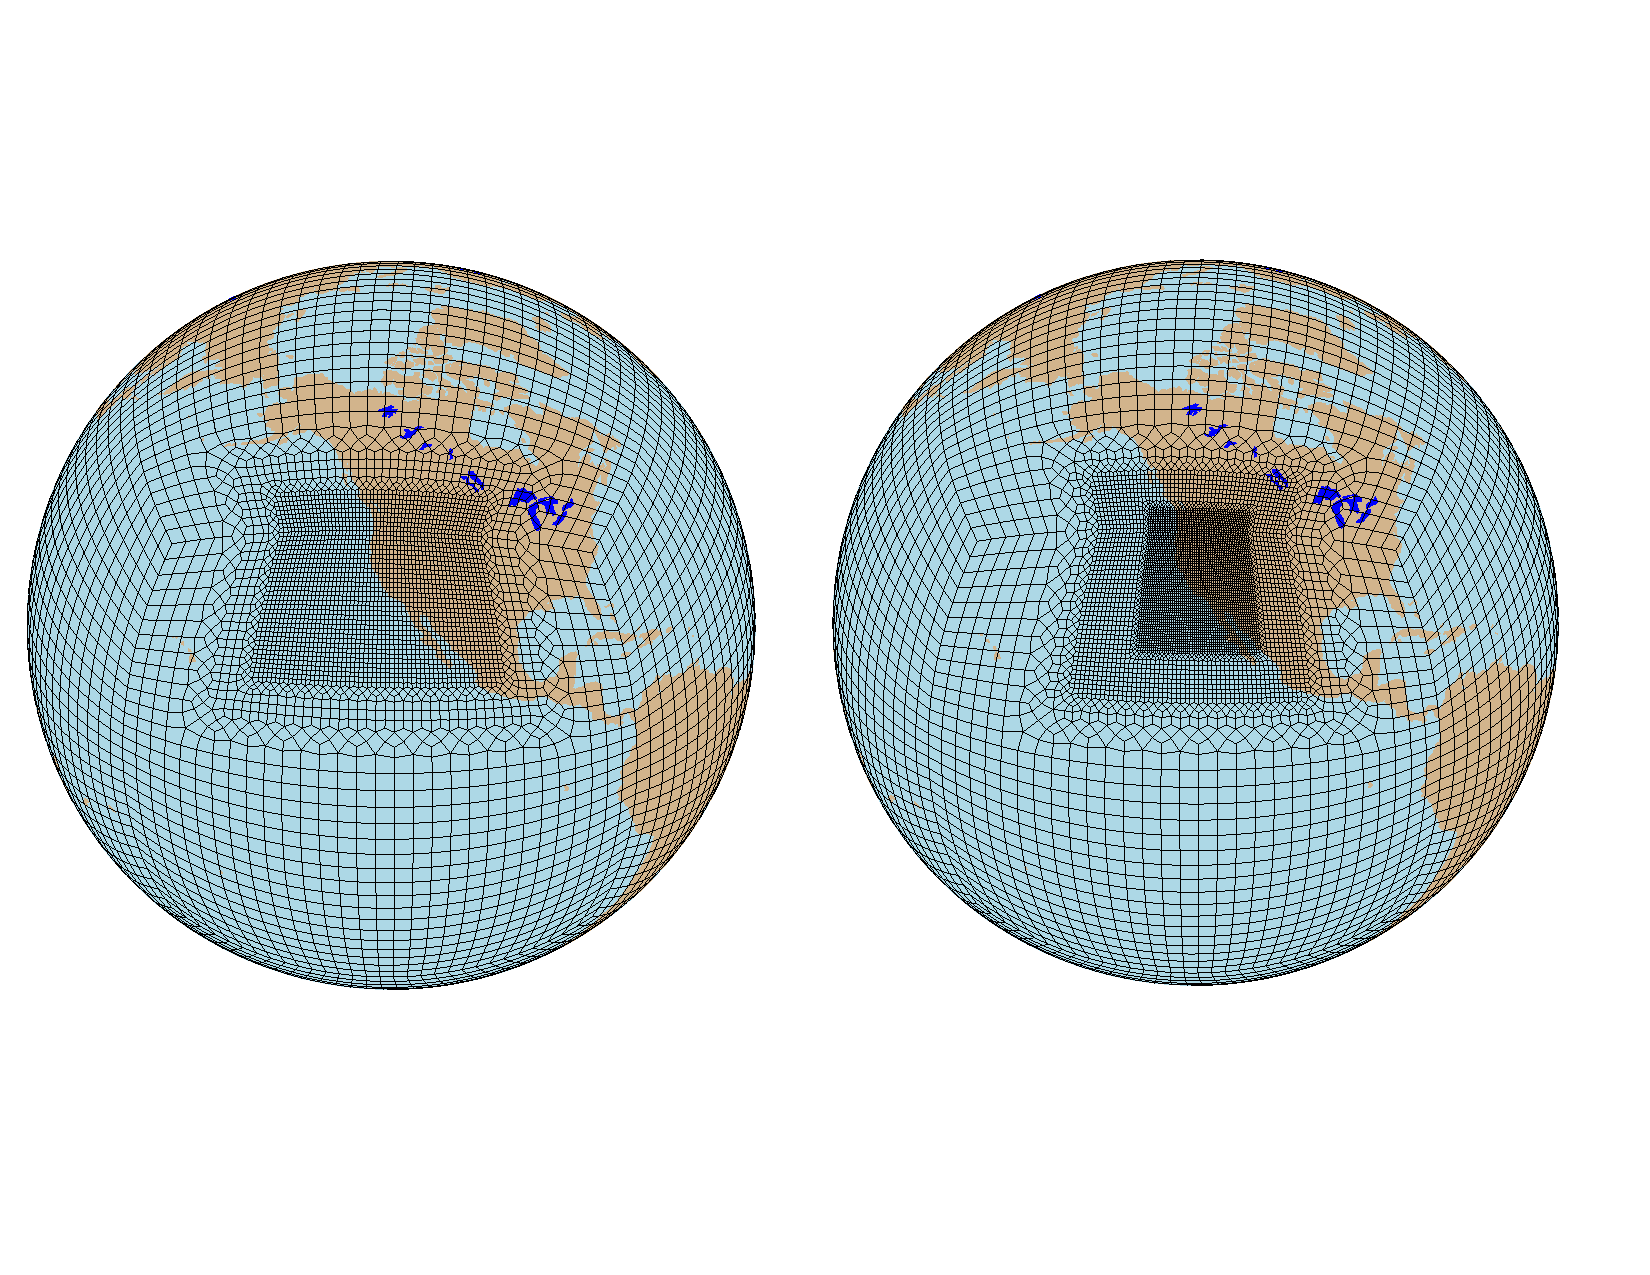
\includegraphics[width=6in]{varres-cesm_gridmesh.pdf}
\end{center}
\caption{Grid meshes for the two varres-CESM simulations.} \label{fig:varres-CESM_map}
\end{figure}

%Approximate regional resolution for the computational grids used in varres-CESM simulations.  The dashed lines and solid lines correspond to the outer boundary and inner boundary of the transition region.

\begin{figure}
\begin{center}
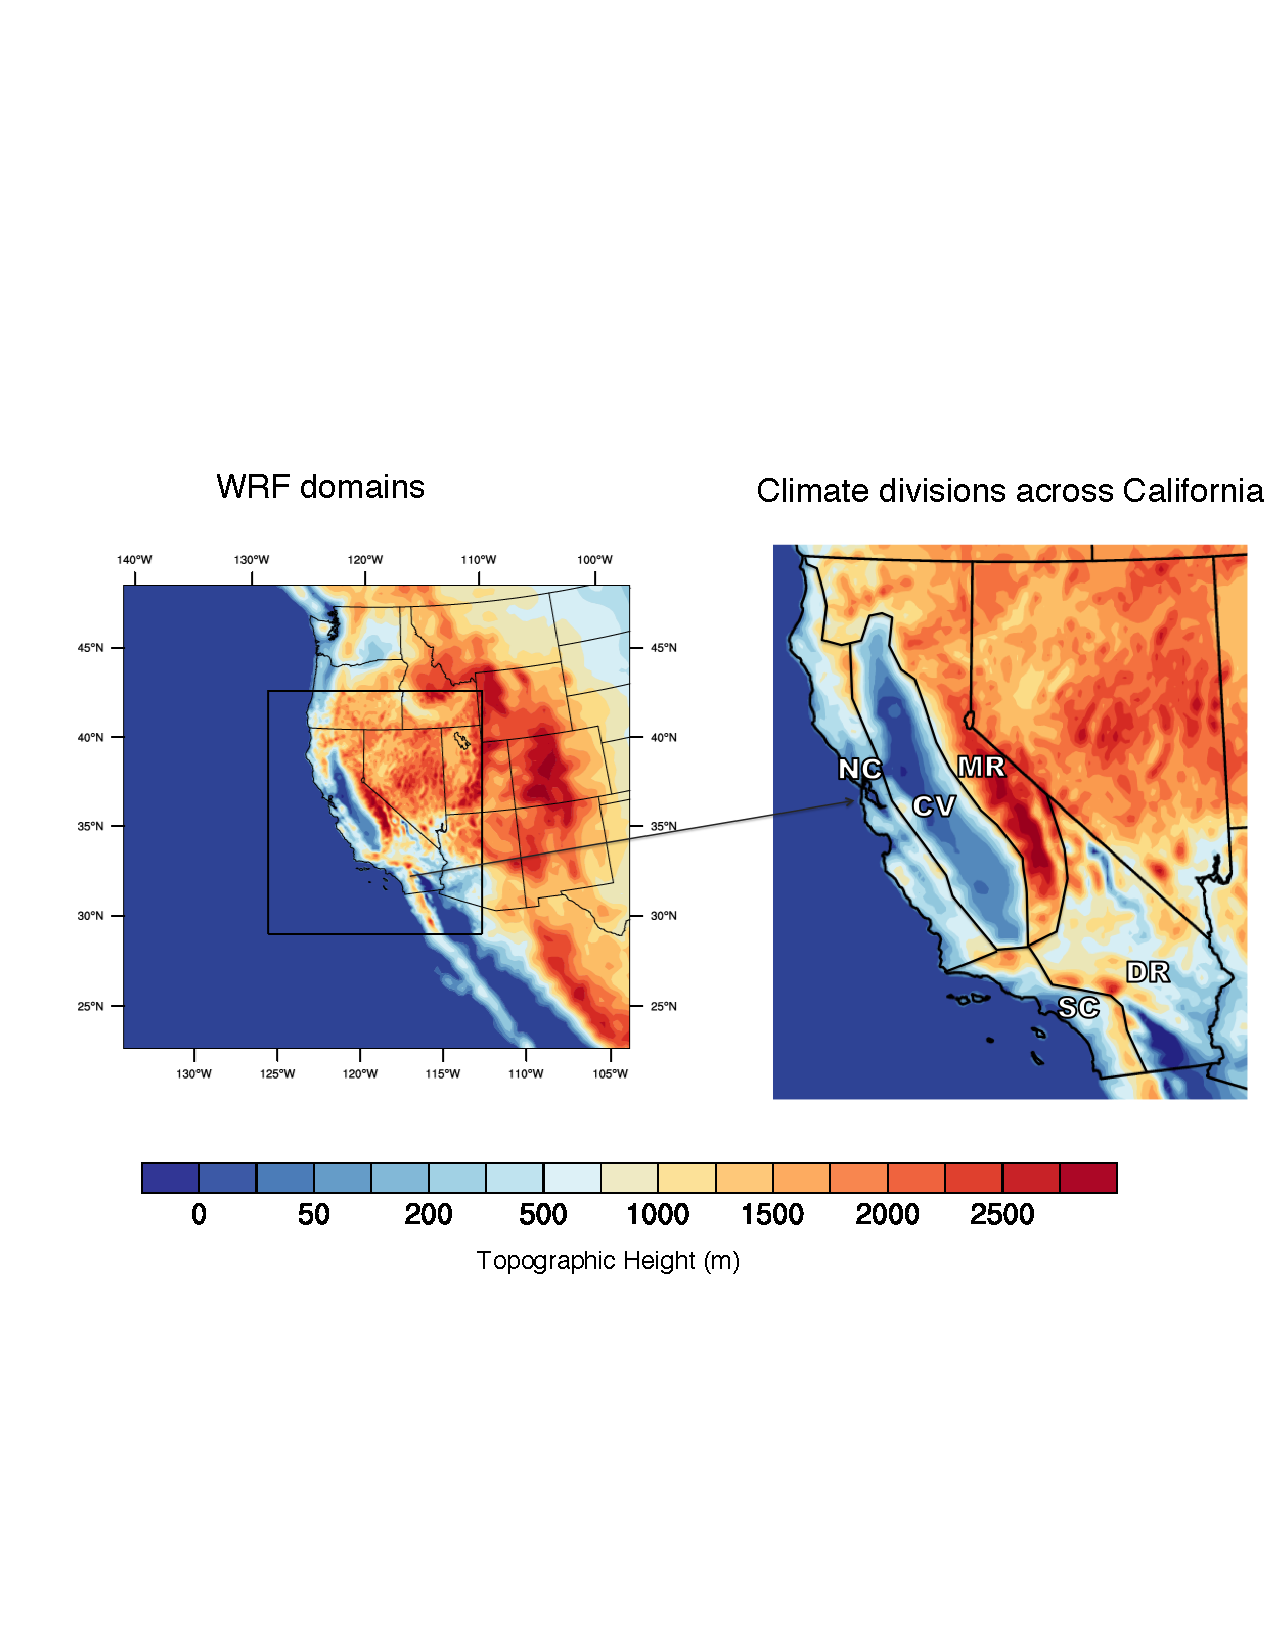
\includegraphics[width=6in]{wrf_domains.pdf}
\end{center}
\caption{Domains of WRF simulations (left) and five climate divisions in California (right) with topography in meters (m). } \label{fig:wrf_domains}
\end{figure}

\begin{figure}
\begin{center}
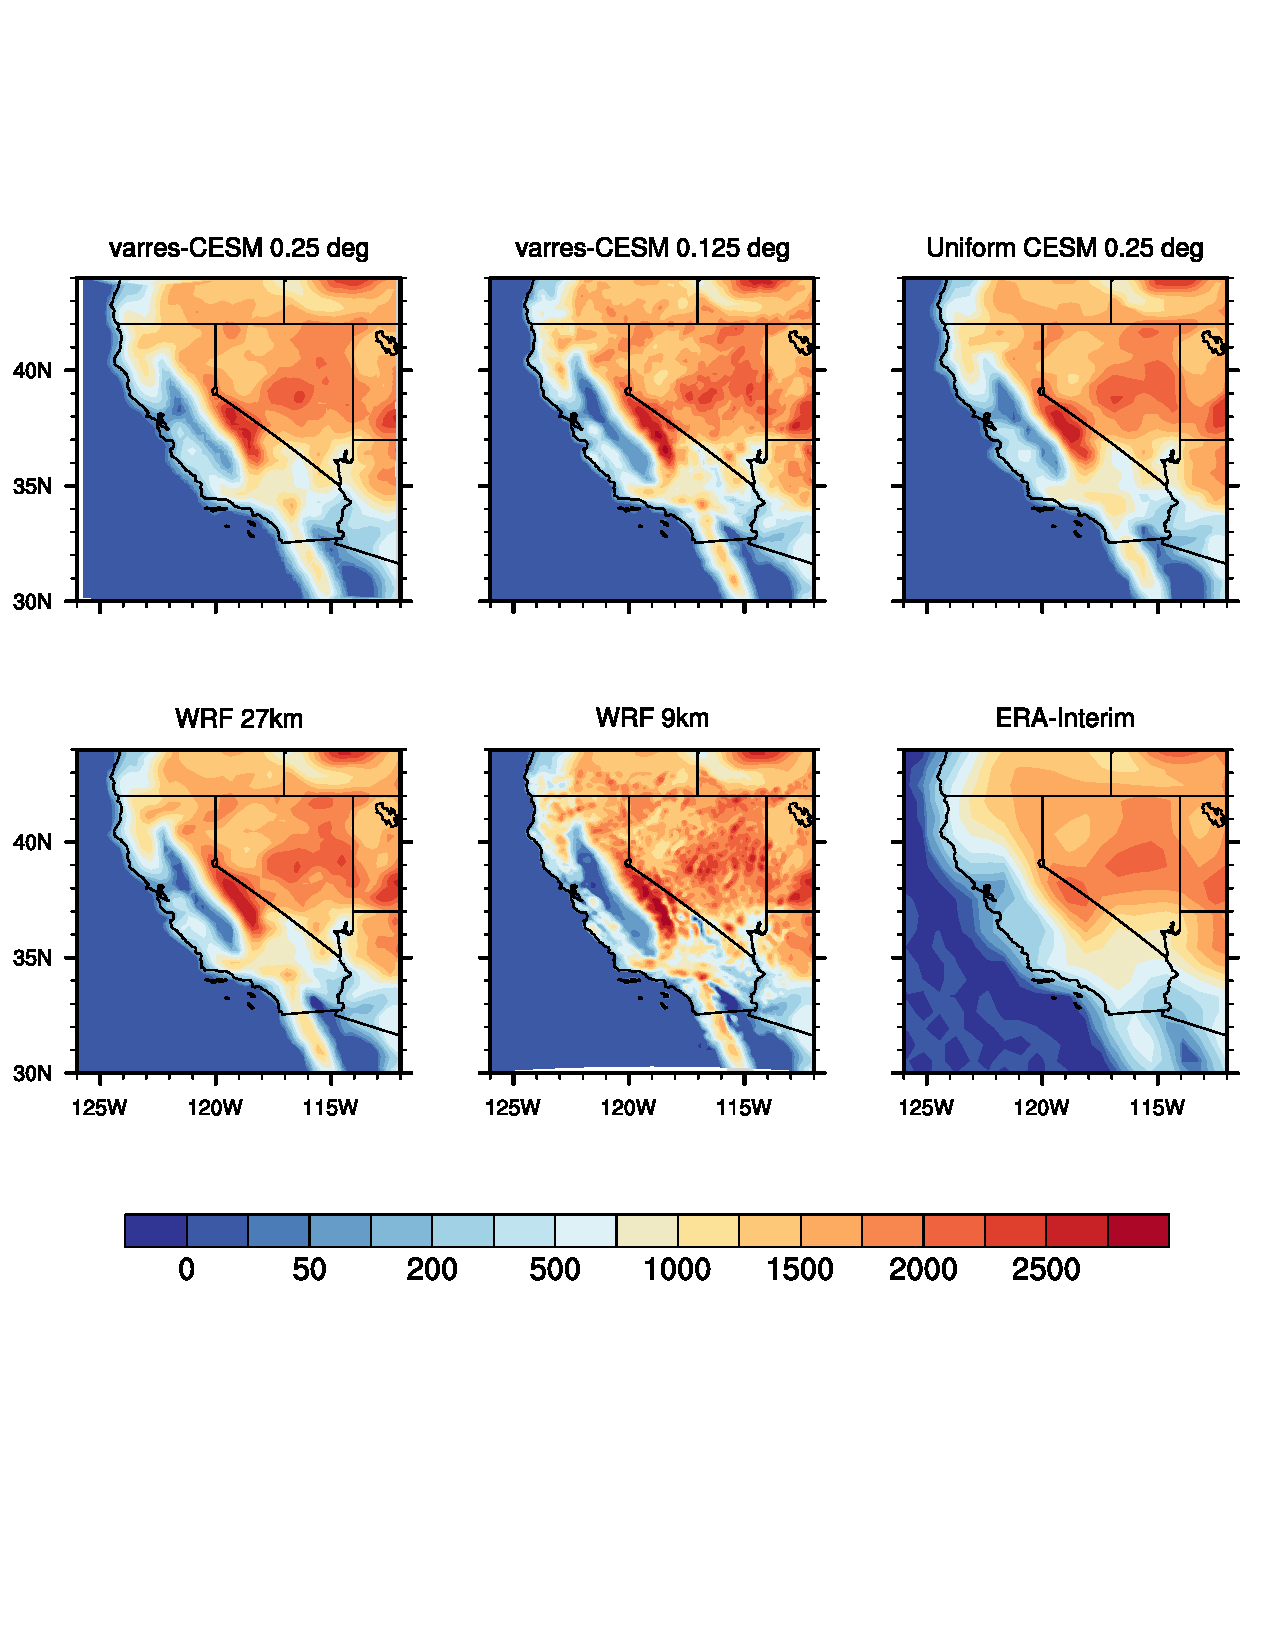
\includegraphics[width=6in]{topo.pdf}
\end{center}
\caption{Topography in meters (m) for (top left to bottom right) varres-CESM 0.25$^\circ$, varres-CESM 0.125$^\circ$, uniform CESM-FV 0.25$^\circ$, WRF 27km, WRF 9km and ERA-Interim ($\sim$80 km).} \label{fig:topo} 
\end{figure}

\begin{figure}
\begin{center}
\includegraphics[width=6in]{t2_JJA.pdf}
\end{center}
\caption{JJA average daily Tmax, Tmin and Tavg from models and reference datasets, and differences between models and PRISM ($^\circ$C). {\color{red}Maybe remove Uniform CESM and move PRISM to the first row at the end.  Place difference color bar somewhere more in line with plots.}} \label{fig:t2_JJA}
\end{figure}

\begin{figure}
\begin{center}
\includegraphics[width=6in]{t2_JJA_std.pdf}
\end{center}
\caption{Sample standard deviation of JJA average daily Tmax, Tmin and Tavg from models and PRISM ($^\circ$C).} \label{fig:t2_JJA_std}
\end{figure}

\begin{figure}
\begin{center}
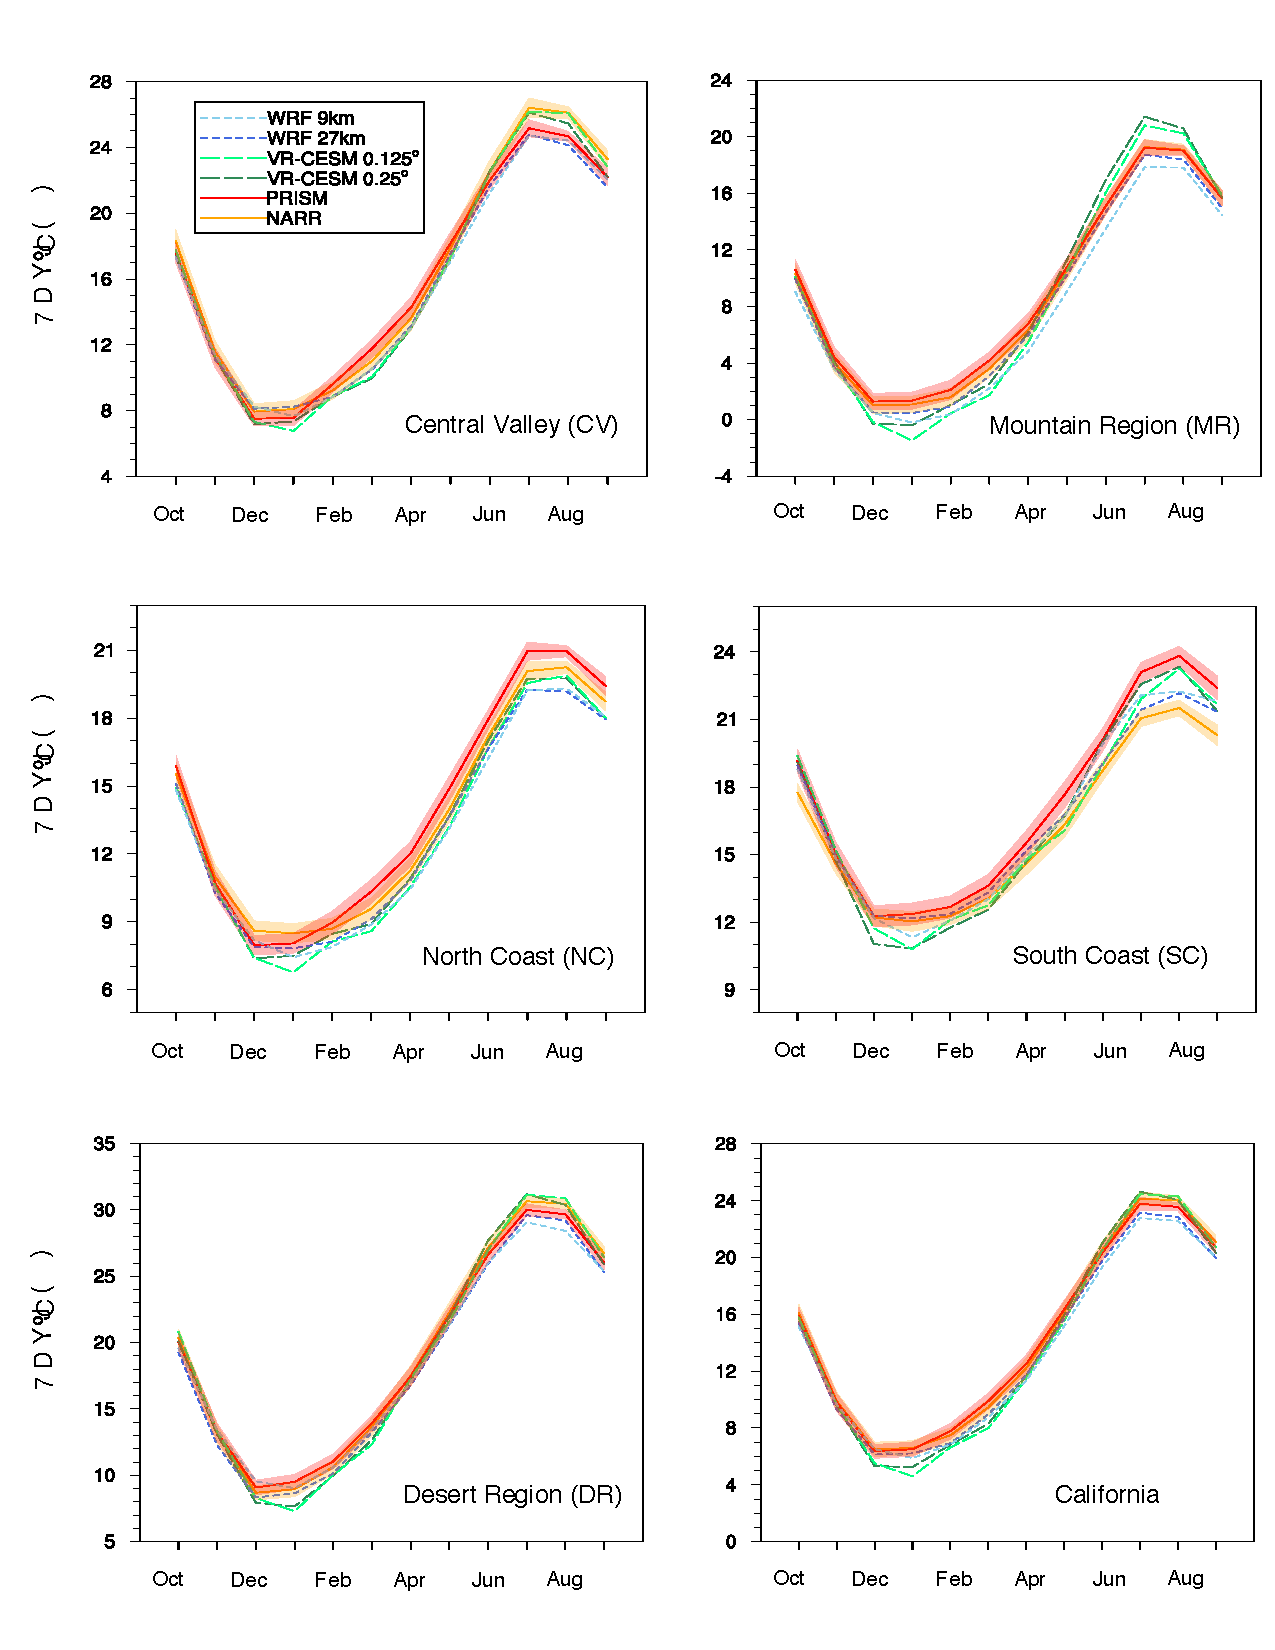
\includegraphics[width=6in]{trd_t2avg_allzones.pdf}
\end{center}
\caption{Seasonal cycle of monthly-average Tavg for each subzone ($^\circ C$).  {\color{red}Can you add the 0.95 confidence interval to PRISM and NARR?}} \label{fig:trd_t2avg_allzones}
\end{figure}

\begin{figure}
\begin{center}
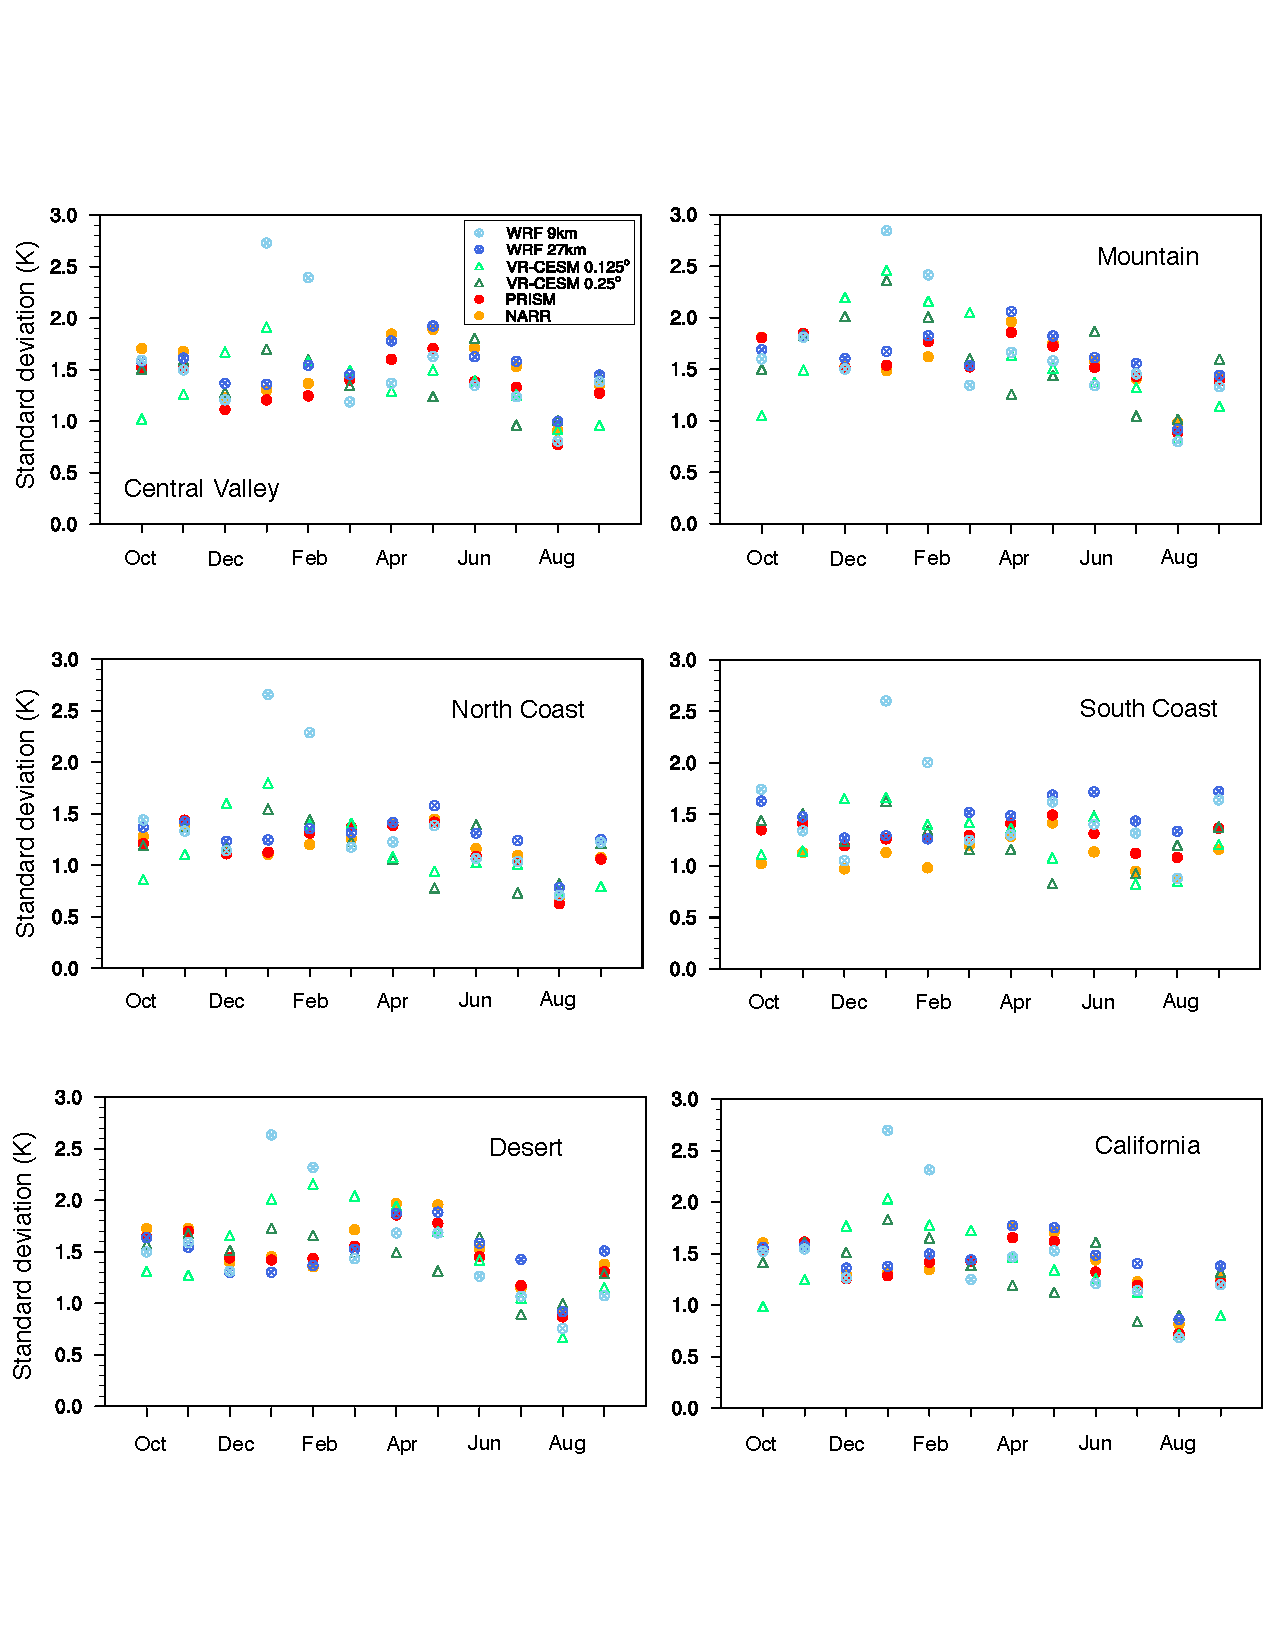
\includegraphics[width=6in]{trd_t2avg_allzones_std.pdf}
\end{center}
\caption{Seasonal standard deviation ($s$) values of monthly-average Tavg for each subzone ($^\circ C$).} \label{fig:trd_t2avg_allzones_std}
\end{figure}


\begin{figure}
\begin{center}
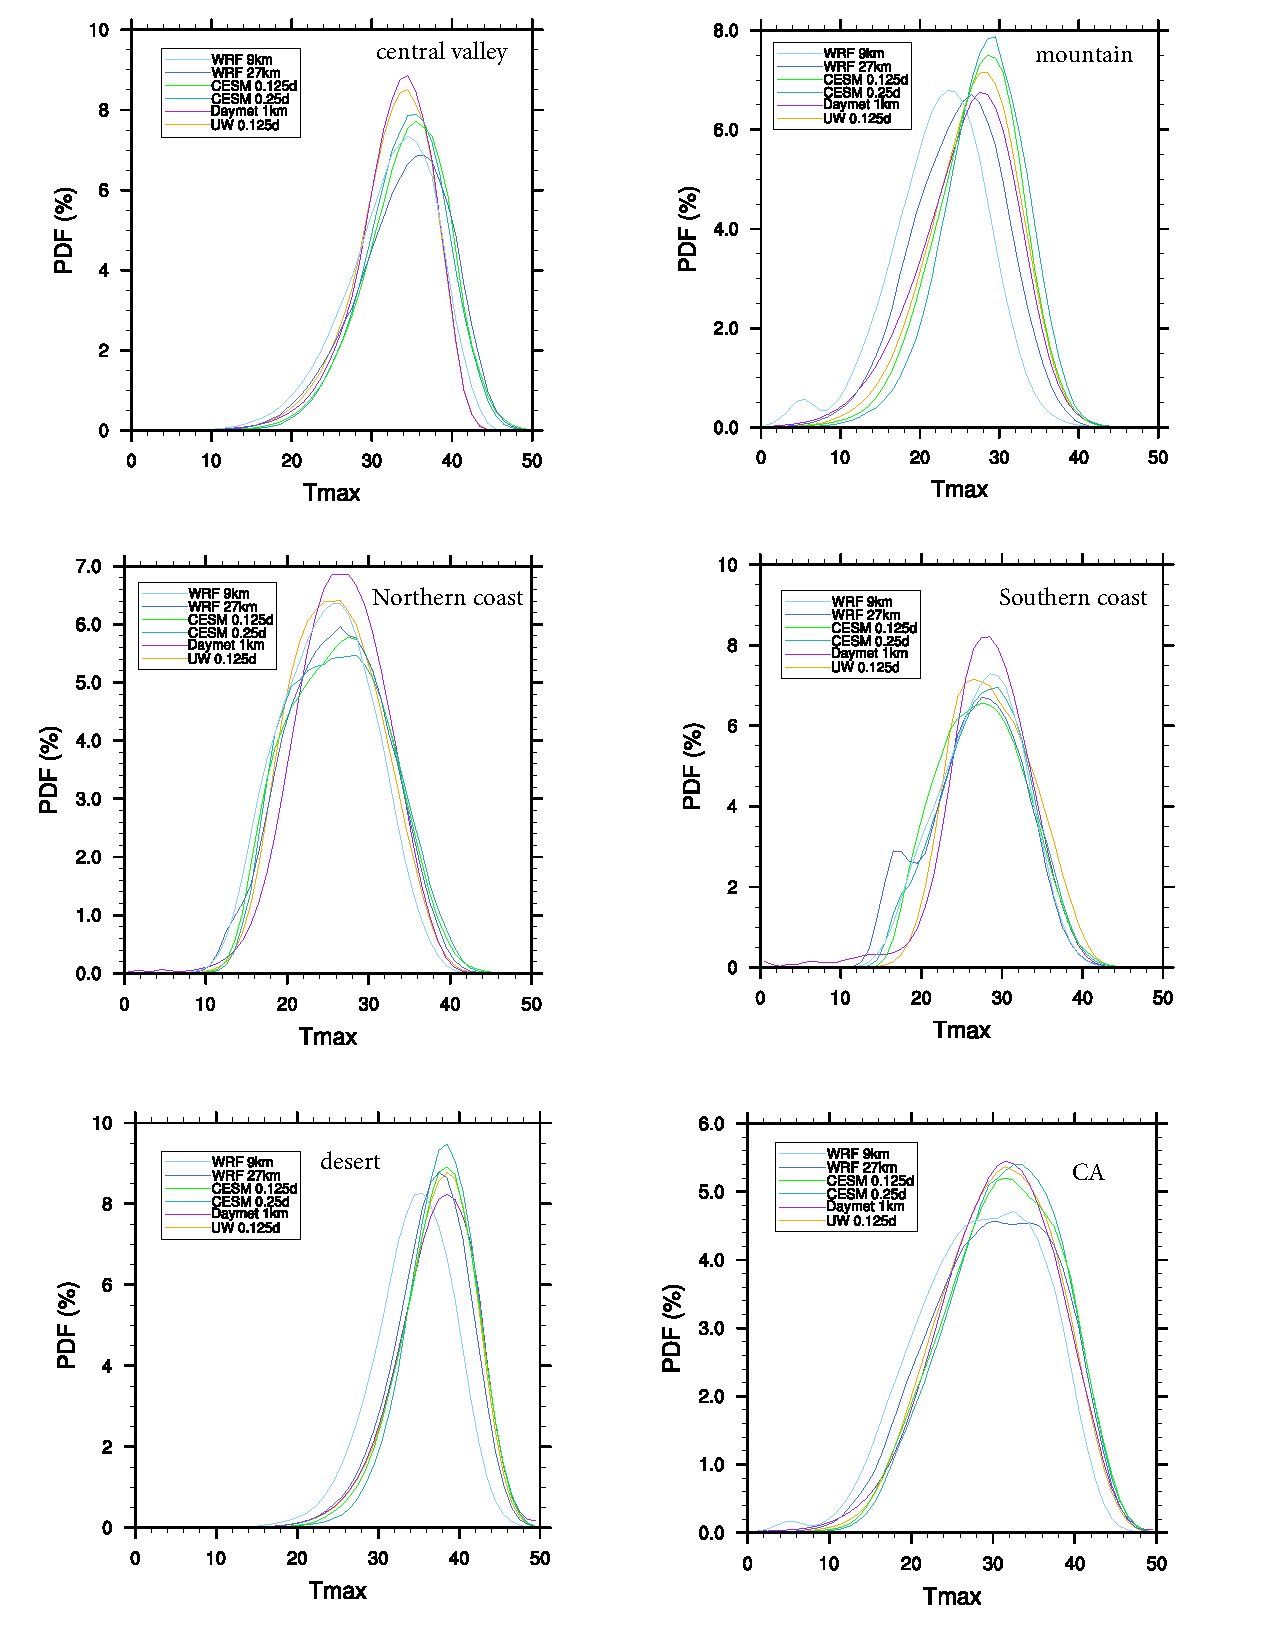
\includegraphics[width=6in]{PDF_t2max_allzones_JJA.pdf}
\end{center}
\caption{Frequency distribution of summer Tmax ($^\circ C$).} \label{fig:PDF_t2max_allzones_JJA}
\end{figure}


\begin{figure}
\begin{center}
\includegraphics[width=6in]{pr_DJF_Annual.pdf}
\end{center}
\caption{Annual and DJF precipitation from models and reference datasets, and differences between models and PRISM (mm/d). {\color{red}Mask out ocean in WRF 9km - PRISM plot.}} \label{fig:pr_DJF_Anuual}
\end{figure}

\begin{figure}
\begin{center}
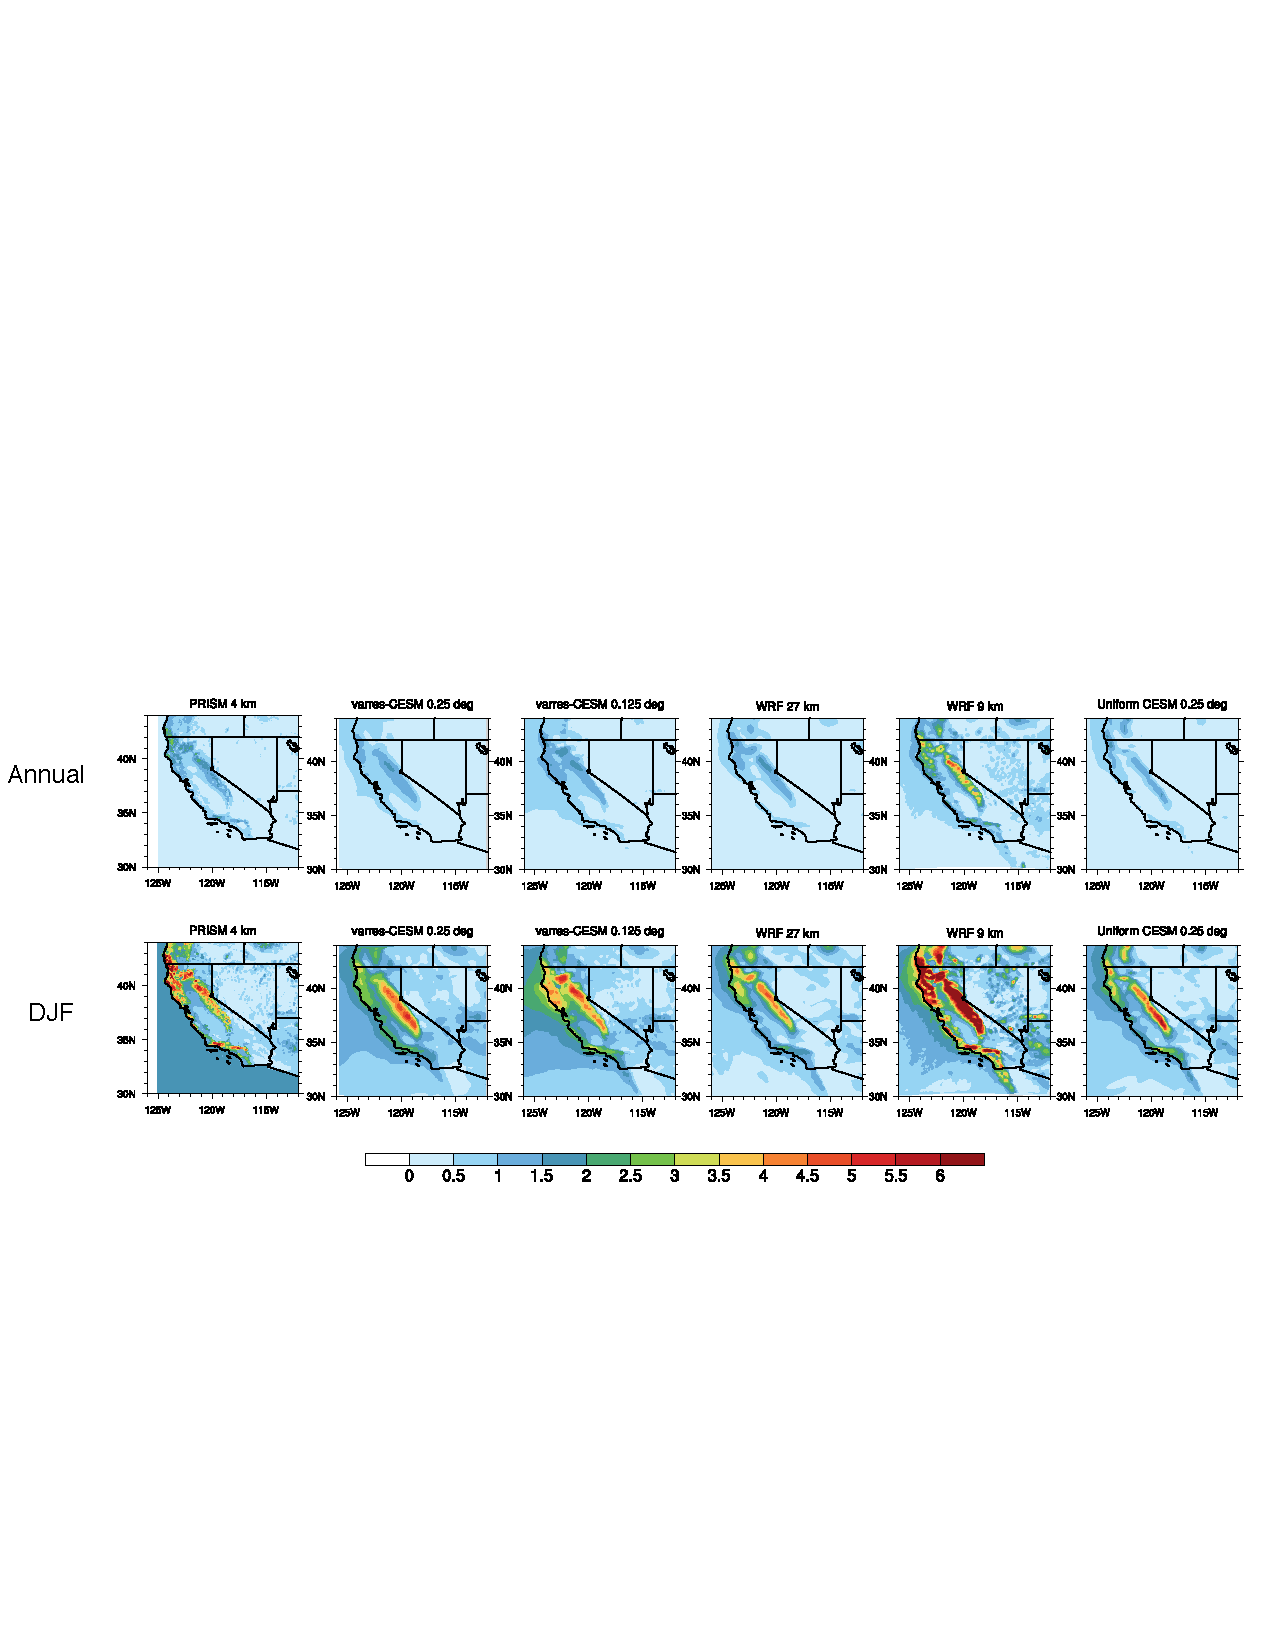
\includegraphics[width=6in]{pr_DJF_Annual_std.pdf}
\end{center}
\caption{Sample standard deviation of Annual and DJF precipitation from models and PRISM (mm/d). {\color{red}Move PRISM to left-hand-side.}} \label{fig:pr_DJF_Annual_std}
\end{figure}

\begin{figure}
\begin{center}
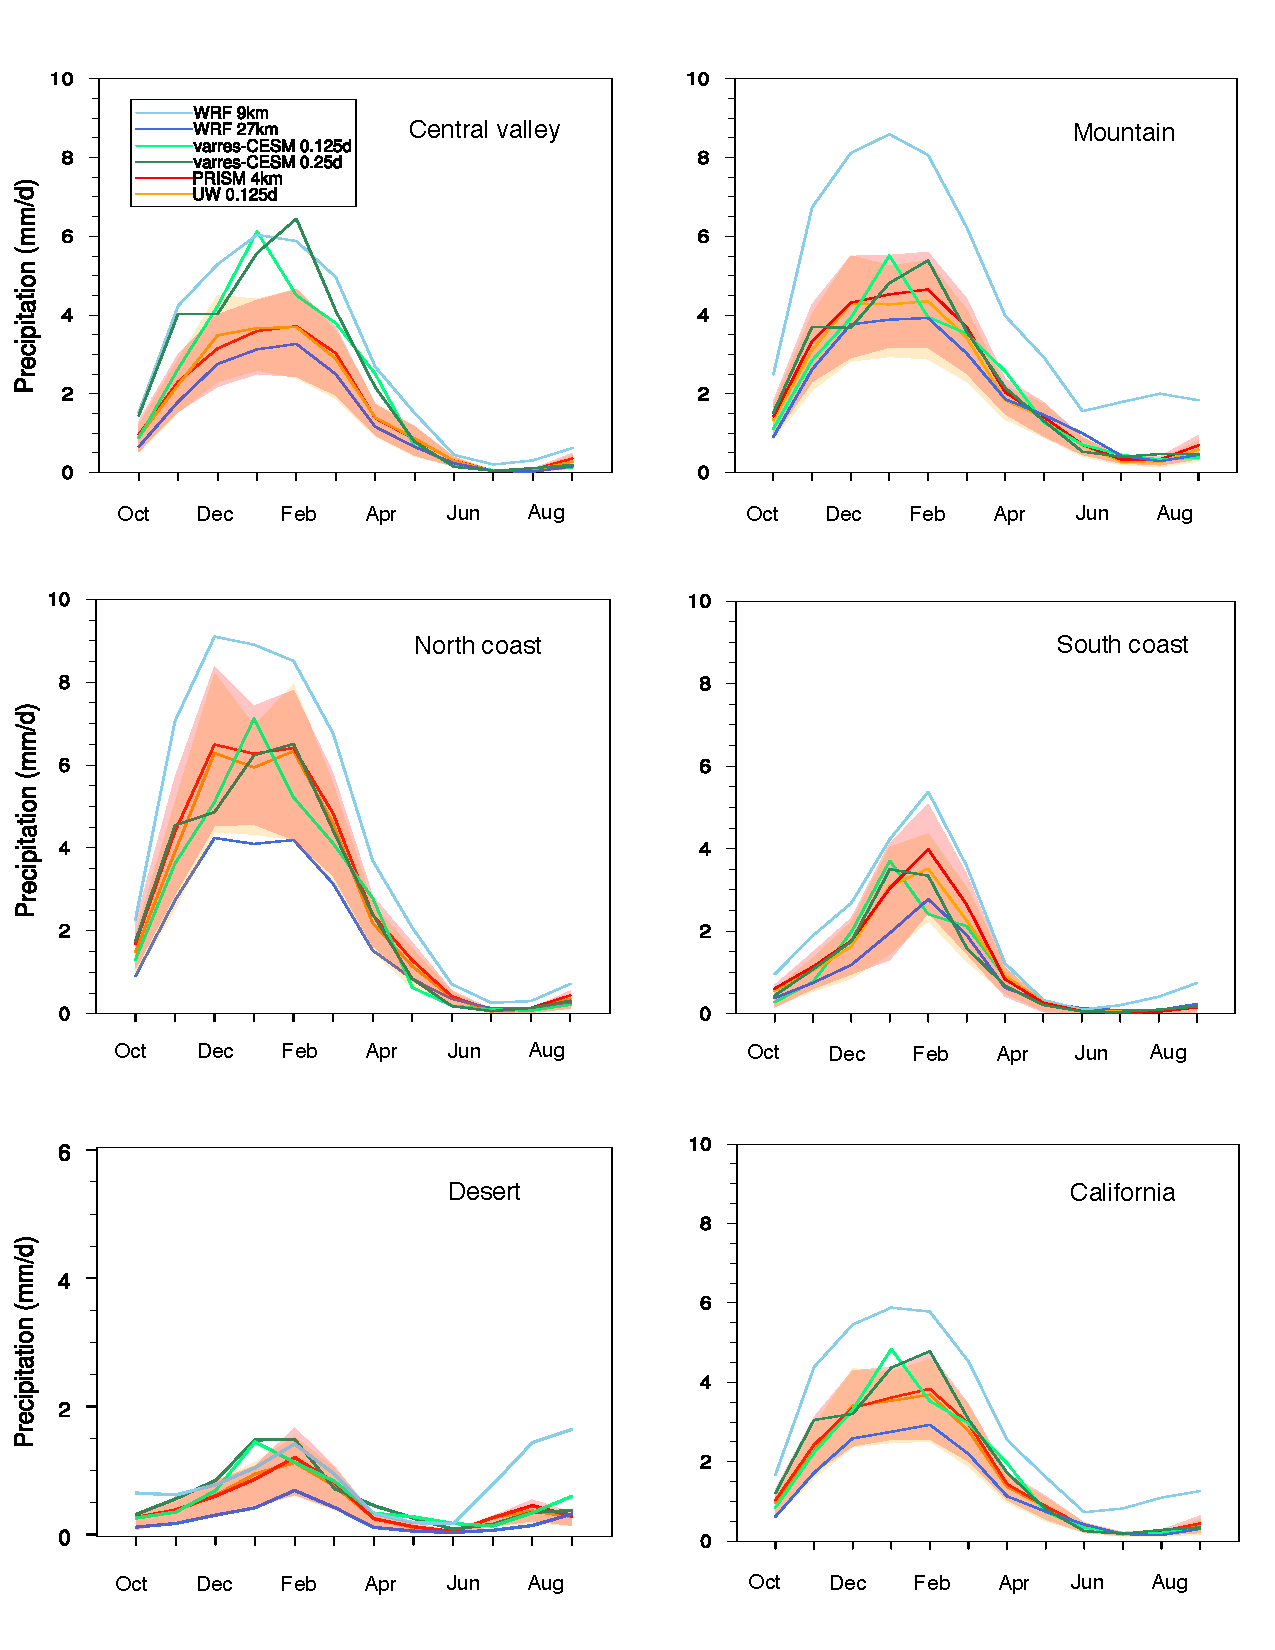
\includegraphics[width=6in]{trd_pr_allzones.pdf}
\end{center}
\caption{As Figure 6, but for monthly-average total precipitation (mm/d).  {\color{red}Can you add the 0.95 confidence interval to PRISM and UW?}} \label{fig:trd_pr_allzones}
\end{figure}

\begin{figure}
\begin{center}
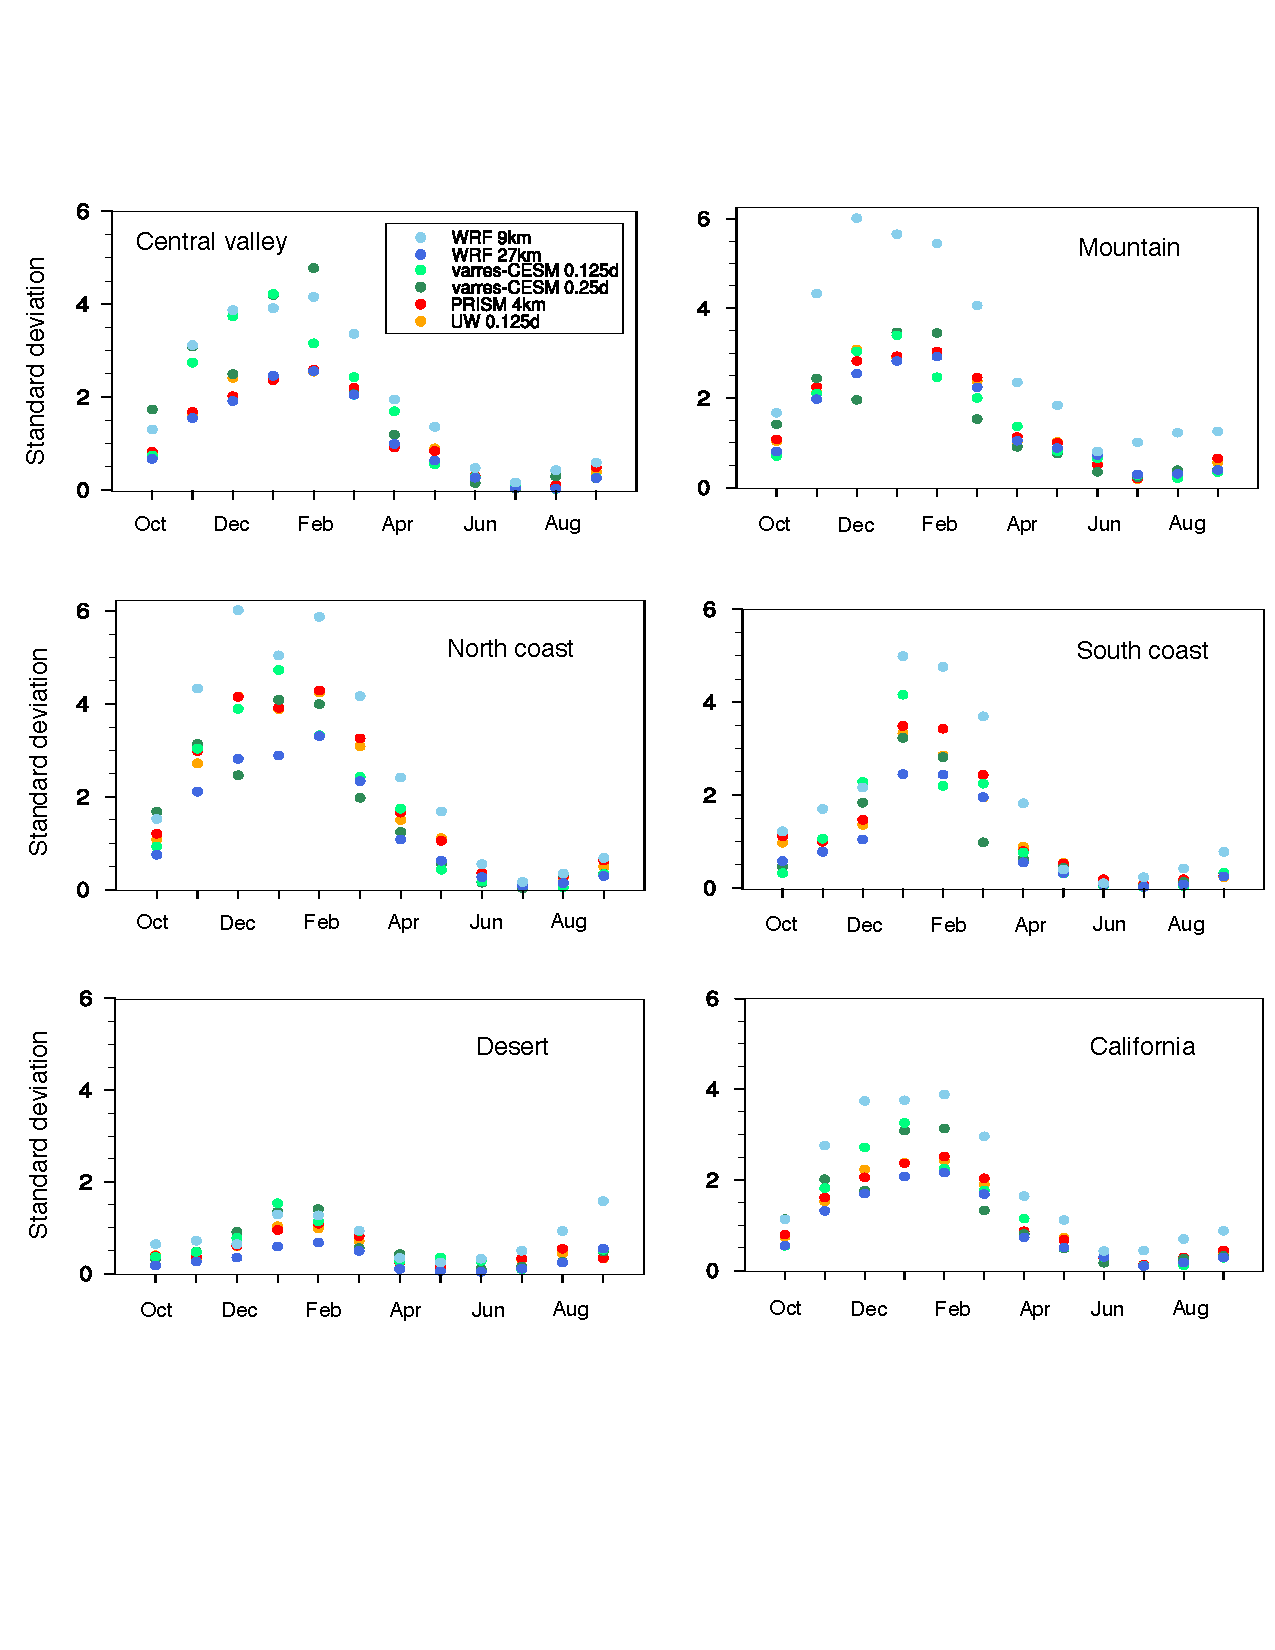
\includegraphics[width=6in]{trd_pr_allzones_std.pdf}
\end{center}
\caption{As Figure 7, but for monthly-average total precipitation (mm/d).} \label{fig:trd_pr_allzones_std}
\end{figure}

\begin{figure}
\begin{center}
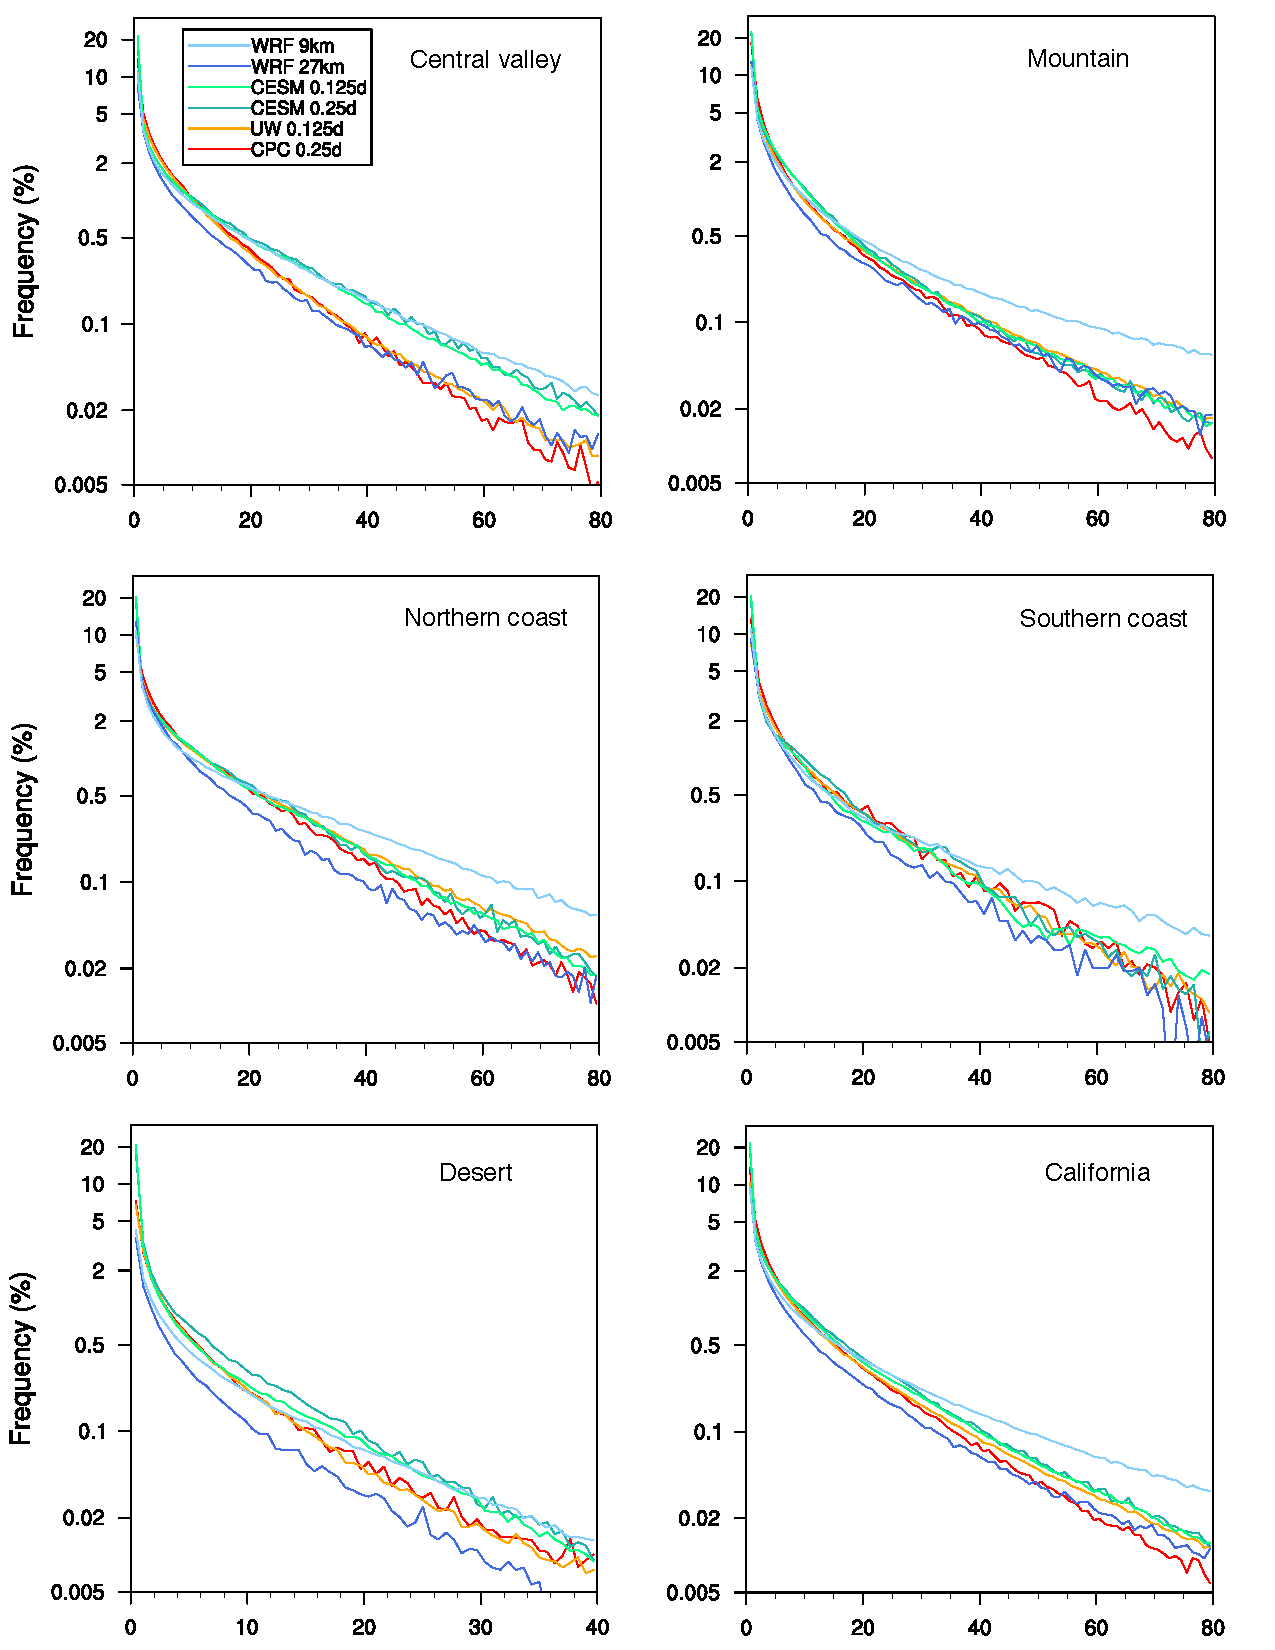
\includegraphics[width=6in]{PDF_pr_allzones_DJF.pdf}
\end{center}
\caption{Frequency distribution of winter Pr, the unit of x-axis is mm/d (note that the vertical scale is logarithmic).} \label{fig:PDF_pr_allzones_DJF}
\end{figure}

\begin{figure}
\begin{center}
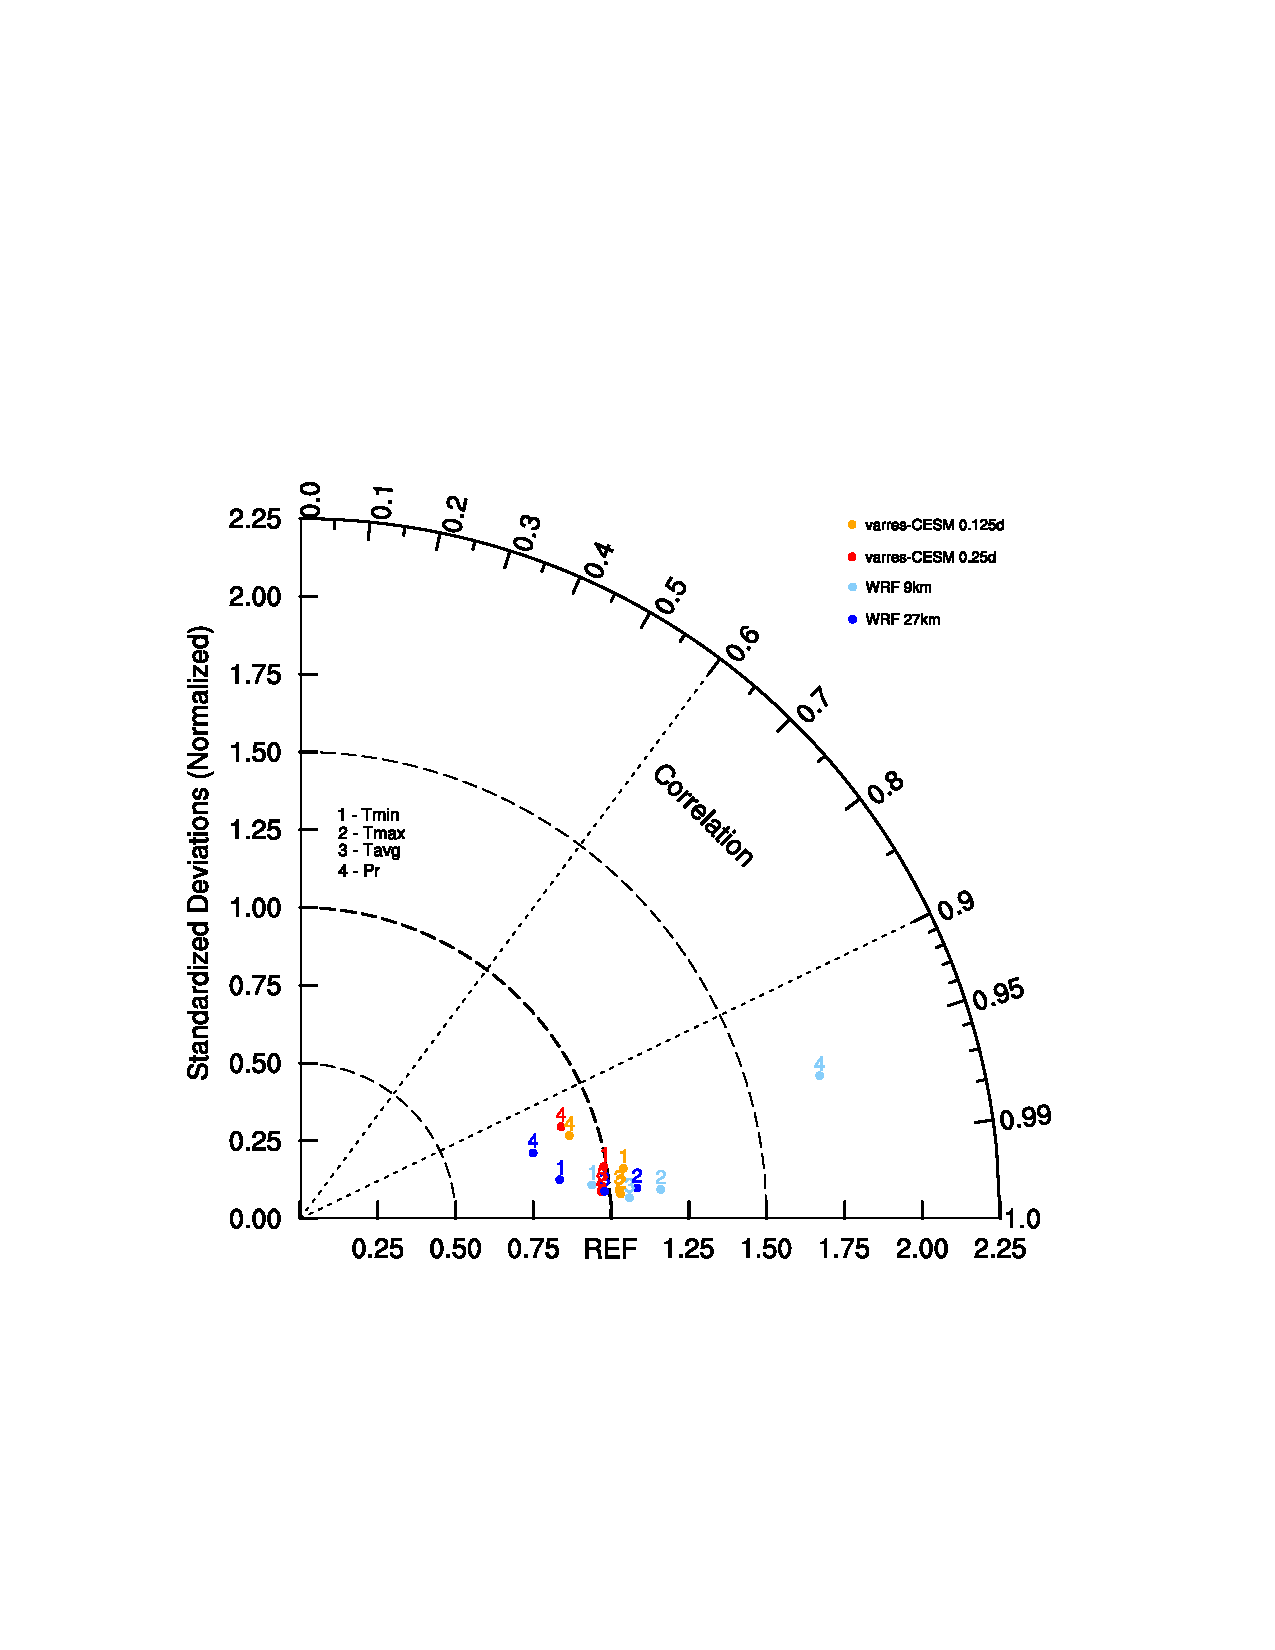
\includegraphics[width=6in]{taylor_diagram.pdf}
\end{center}
\caption{Taylor diagram of annual climatology for the entire California region, using the PRISM dataset as reference.} \label{fig:taylor_diagram}
\end{figure}

%upload grid, namelist file and settings files so that people can reproduce 
%probably at the last to come up a table that containing all the diagnostic variables and the corresponding model that works best. maybe not.


%%%%%%%%%%%%%%%%%%%%%%%%%%%%%%%%%%%%%%%%%%%%%%%%%%%%%%%%%%%%%%%%%%%%%
% END OF AMSPAPER.TEX
%%%%%%%%%%%%%%%%%%%%%%%%%%%%%%%%%%%%%%%%%%%%%%%%%%%%%%%%%%%%%%%%%%%%%

%%%%%%%%%%%%%%%%%%%%%

\end{document}
